%%%%%%%%%%%%%%%%%%%%%%%%%%%%%%%%%%%%%%%%
%% MCM/ICM LaTeX Template %%
%%%%%%%%%%%%%%%%%%%%%%%%%%%%%%%%%%%%%%%%

\documentclass{mcmthesis}
\mcmsetup{
	tstyle=\color{red}\bfseries,
	tcn = 2624654, problem = C,
	sheet = true, titleinsheet = false, keywordsinsheet = true,
	titlepage = false, abstract = true
}
\setlength{\headheight}{14pt}
\usepackage{enumitem} % <--- 【关键】必须引入这个宏包来控制列表间距
\usepackage{newtxtext,newtxmath}
\usepackage{indentfirst}
\usepackage{lipsum}
\usepackage{tabularx}
\usepackage{enumitem}
\usepackage{float}
\usepackage{setspace}
\usepackage{subcaption}
% 如果模板里已经加载了 algorithm，这里将其强制取消定义，
% 避免和下面的 algorithm2e 打架
\makeatletter
\let\algorithm\relax
\let\algorithm\undefined
\let\listofalgorithms\undefined
\makeatother
\usepackage{tabularx}

% -------------------------------------------
\usepackage{booktabs}  % 用于三线表
\usepackage{url}       % 用于处理网址
\usepackage{hyperref}  % 用于生成可点击的链接（可选）
\usepackage[ruled,vlined]{algorithm2e} % 加载更强大的算法包
\usepackage{booktabs}
% 这一步是关键！加载 Times New Roman 风格的文本和数学字体
\usepackage{newtxtext}
\usepackage{newtxmath}
\usepackage{fancyhdr}
\usepackage{lastpage} % 用于获得总页数
\usepackage{tocloft}  % 专门用于定制目录样式的宏包
\usepackage{newtxtext} % 文本字体用 Times
\usepackage{newtxmath} % 数学字体用 Times (优化版)
% 2. 设置目录标题样式
\renewcommand{\contentsname}{\bfseries\Large Contents} % 目录标题加粗、变大
\renewcommand{\cfttoctitlefont}{\bfseries\Large} 
\renewcommand{\cftaftertoctitle}{\vspace{1em}} % 标题和列表之间的间距

% 3. 设置一级标题 (Section) 的样式
\renewcommand{\cftsecfont}{\bfseries}       % 序号和标题加粗
\renewcommand{\cftsecpagefont}{\bfseries}   % 页码加粗
\renewcommand{\cftsecleader}{\cftdotfill{\cftdotsep}} % 【关键】强制一级标题显示点线

% 4. 设置二级标题 (Subsection) 的样式
\renewcommand{\cftsubsecfont}{\normalfont}  % 正常字体（不加粗）
\renewcommand{\cftsubsecpagefont}{\normalfont} % 页码正常字体

% 5. 调整行距 (可选，根据需要调整)
\setlength{\cftbeforesecskip}{0.5em}    % 一级标题前的间距
\setlength{\cftbeforesubsecskip}{0.2em} % 二级标题前的间距
\usepackage{graphicx}
\usepackage{tabularx}

\setcounter{tocdepth}{2}
\usepackage{float}
\title{The \LaTeX{} Template for MCM Version \MCMversion}
\author{\small \href{https://www.latexstudio.net/}
	{\includegraphics[width=7cm]{mcmthesis-logo}}}
\date{\today}
\usepackage{setspace} 
\begin{document}

% --- 替换原来的 abstract 部分 ---
\begin{abstract}
	\setlength{\parindent}{2em}        % 段首缩进（像示例那样）
	\setlength{\parskip}{1pt}          % 段间不额外加空白（空白就没了）

The competitive tension in DWTS stems from the interplay between judges' merit-based evaluations and audience popularity votes. However, the longstanding lack of transparency in fan voting has turned the elimination mechanism into a "black box," sparking controversy over "popularity overpowering skill." Relying solely on judges' scores and elimination outcomes makes it difficult to uniquely pinpoint the hidden variable of fan sentiment. This paper constructs a multidimensional mathematical framework to reconstruct latent fan sentiment flows through reverse inference, seeking the optimal "dynamic equilibrium point" between technical expertise and audience engagement.

\smallskip
\textbf{For Task 1}, we formulate vote restoration as an \textbf{ill-posed inverse problem} and propose a \textbf{Hierarchical Bayesian Reconstruction framework (HBR-Vote)}. By coupling hierarchical priors with rule-consistency constraints, and performing posterior inference using an \textbf{Adaptive Constrained MCMC sampler (ACMH)}, we draw samples from the full posterior to recover weekly fan vote shares with quantified uncertainty. Empirically, our reconstruction attains \textbf{99.62\%} elimination-consistency over 34 seasons, with an average certainty score of \textbf{0.644}. Moreover, uncertainty surges from \textbf{0.3} to \textbf{1.1} as the contestant pool shrinks, indicating increasingly volatile fan behavior and higher predictive difficulty in later stages.

\smallskip
\textbf{For Task 2}, we conduct a comparative analysis between the \textbf{Rank system} and the \textbf{Percentage system}. Statistical tests show that the Percentage system is \textbf{13.6\%} more sensitive to fan intent, making extreme outliers more likely to override technical standards. To mitigate this, we model the ``Judge's Save'' as a nonlinear \textbf{circuit breaker}. Historical backtesting demonstrates that the hybrid mechanism achieves a \textbf{Controversy Suppression Rate (CSR) of 89.5\%} and rectifies controversial outcomes (e.g., ``Bobby Bones''). Overall, it filters popularity-driven weak performers while preserving meaningful fan participation, providing a practical path for future rule evolution.

\smallskip
\textbf{For Task 3}, we quantify how professional partners and celebrity traits affect judges and fans differently via a two-layer attribution framework: we first apply \textbf{Linear Mixed Effects (LME)} to remove season-level fixed effects, then integrate \textbf{LightGBM} with \textbf{SHAP} to explain nonlinear contributions. The results reveal a clear \textbf{preference decoupling} ($r=0.47$): judges emphasize \emph{technical auditing}---the pro partner's win-rate effect is about \textbf{2.1$\times$} stronger on the judges' side, and athletes enjoy a technical premium ($\beta_{\text{judge}} \approx 0.42$). In contrast, fans favor \emph{identity narratives}, with reality-TV stars showing a distinctive relatability premium ($\beta_{\text{fan}} \approx 0.38$). We further identify an \textbf{aging-buffer} interaction: veteran pro partners significantly mitigate the survival disadvantage associated with older celebrities.

\smallskip
\textbf{For Task 4}, we developed the \textbf{Dynamic Weighted Comprehensive Scoring Model (DWCSM)}: introducing a "funnel strategy" that progressively increases technical weighting throughout the competition schedule to ensure champion selection reverts to professional standards. To mitigate the power-law bias in fan voting, we employed an \textbf{EMA} progress index to capture "growth narratives." Retrospective simulations for Season \textbf{27} adjusted the ranking of a controversial contestant to 4th place, achieving a Pareto improvement: restoring judging authority while preserving program drama and audience impact.

Finally, we synthesize all analyses into a compact, data-driven decision-support framework for refining DWTS voting rules and scoring strategies.
% 关键词
\begin{keywords}
	fan vote reconstruction; hierarchical Bayesian model; controversy suppression rate; 
\end{keywords}
\end{abstract} 		
\begingroup
\setlength{\topsep}{0pt}
\setlength{\partopsep}{0pt}
\setlength{\parskip}{0pt}
\maketitle
\endgroup
\thispagestyle{empty}


\tableofcontents      % 生成目录
\thispagestyle{empty} % 【关键】强制第2页（目录页）不显示页码
\newpage

\setcounter{page}{3}
\section{Introduction}
\subsection{Problem Background} 
"Dancing with the Stars" (DWTS) stands as a global cultural phenomenon, harmonizing professional artistic expression with mass public engagement. The show’s elimination mechanism relies on aggregating expert judge scores and fan votes. However, this dual-evaluation system has historically struggled to balance meritocracy with popularity. The inherent variance imbalance between high-precision judge scores and heavy-tailed fan distribution has occasionally allowed technically weaker contestants to secure controversial victories, necessitating repeated algorithmic reforms from rank-based to percentage-based systems. With fan voting data strictly confidential, the challenge lies in mathematically deciphering the "black box" to evaluate whether the current rules truly select the best dancer. This paper explores the latent distribution of fan votes through inverse modeling and offers in-depth insights into how aggregation algorithms should evolve to optimize the equilibrium between competitive fairness and entertainment value.

\subsection{Clarifications and Restatements}
\begin{itemize}
\setlength{\itemsep}{0pt}   % 列表项间距归零
\setlength{\parskip}{0pt}   % 段落间距归零
\setlength{\parsep}{0pt}    % 内部间距归零

\item Task 1: Latent Variable Reconstruction. Develop a model to reconstruct unobservable fan votes and quantify uncertainty to validate consistency with historical eliminations.

\item Task 2: Comparative Analysis. Leveraging Task 1 results, compare Rank-Based vs. Percentage-Based systems and simulate the impact of the ``Judges' Save'' on historical controversies.

\item Task 3: Driver Attribution. Incorporating Task 1 estimates, quantify the influence of professional partners and demographics on both technical scores and fan popularity.

\item Task 4: System Optimization. Design an improved scoring mechanism that optimizes the balance between meritocratic fairness and fan engagement for future seasons.

\item Task 5: Strategic Advisory. Synthesize findings into a memo for producers, providing actionable recommendations on voting rules.
\end{itemize}
\vspace{-0.6em}
\subsection{Model Overview} 

\begin{figure}[htbp]
	\centering
	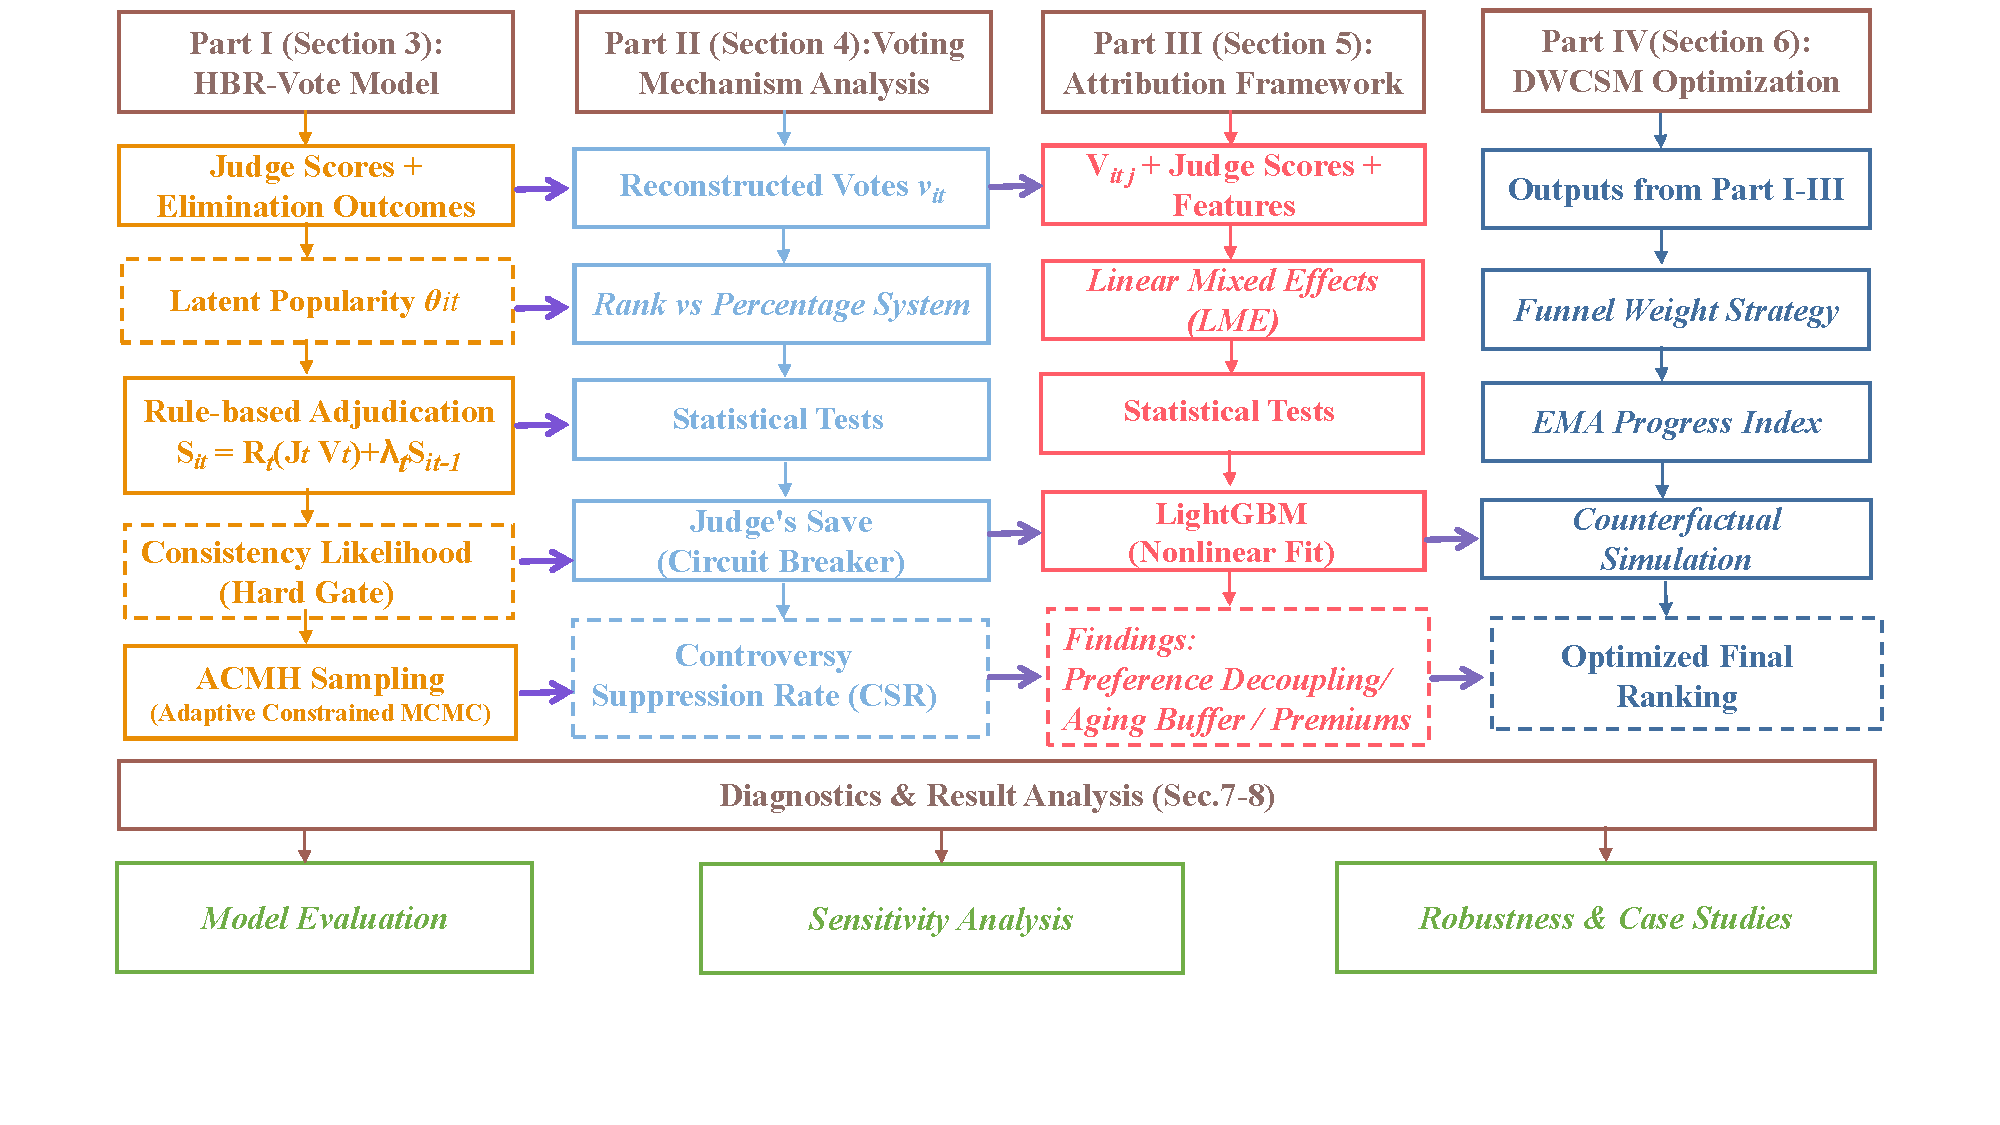
\includegraphics[width=0.78\textwidth]{3.pdf}
	\vspace{-1.6em}
	\caption{Model Overview}
\end{figure}

\section{Preparation for Modeling}
\subsection{Model Assumptions} 
\begin{itemize}
	\item During non-elimination weeks, system states are strictly preserved rather than reset. Elimination constraints for the following week are defined by cumulative performance states across the entire cycle, not by single-week performance.
	
	\item Fan bases exhibit random fluctuations yet possess significant short-term inertia. Unlike traditional Gaussian white noise, we model voting perturbations as following a power-law distribution. This implies that a tiny fraction of ``superstars'' can command the vast majority of votes.
	
	\item All data are authentic.
\end{itemize}
\vspace{-0.4cm}
\subsection{Notifications} 
\vspace{-0.5cm}
\begin{table}[h]
	\caption{Significant symbols in this paper} \vspace{-9mm}
	\begin{center}
		\begin{tabular}{cl}
			\toprule[1.5pt]
			\textbf{Symbols} & \textbf{Description} \\
			\midrule[0.6pt]
			$i, t$ & Indices representing the $i^{th}$ contestant and the $t^{th}$ competition week\\
			$\Omega_t$ & The set of \textbf{active contestants} remaining in the competition at week $t$\\
			$J_{i,t}$ & The observable \textbf{judge score} sum received by contestant $i$ at week $t$\\
			$\mathbf{V}$ / $v_{i,t}$ & The latent \textbf{fan vote share} (proportion) to be reconstructed\\
			$\theta_{i,t}$ & The \textbf{latent utility state} representing intrinsic popularity, evolving via Random Walk\\
			$\sigma^2_{walk}$ & The variance parameter controlling the volatility of the \textbf{popularity evolution}\\
			$S_{i,t}$ & The \textbf{effective adjudication state} (Total Score) determining elimination risk\\
			$\lambda_t$ & A \textbf{state memory coefficient} handling score carry-over (Redfoo Rule)\\
			$\mathcal{R}_k(\cdot)$ & The \textbf{regime-dependent operator} defining the specific elimination rule for season $k$\\
			$\oplus$ & The \textbf{hybrid decision operator} used in Regime III (Bottom 2 + Judge Save)\\
			$\mathcal{J}_{save}$ & The judge's binary decision variable in the \textbf{Judge's Save} mechanism\\
			$N_k$ & The total number of contestants participating in season $k$ \\
			$T_k$ & The total duration (number of weeks) of season $k$ \\
			\bottomrule[1.5pt]
		\end{tabular}
	\end{center}
	\label{tab:symbol_description}
\end{table}
\vspace{-0.8cm}
\subsection{Data Preprocessing}	
Based on the attachments provided in the question, we aggregated the individual scores from 3-4 judges to calculate 421 contestants' total score and average score. Simultaneously, we computed weekly internal judge rankings and score percentages for contestants to enable cross-season comparability. We also generated elimination identifiers to mark 264 elimination events and recorded the weekly number of remaining contestants as a contest scenario variable. 

The core challenge in data preprocessing lies in handling historical changes to scoring rules: Seasons 1, 2, and 28-34 used a cumulative ranking system (judge ranking + fan ranking, with the highest combined rank eliminated), while Seasons 3-27 switched to a cumulative percentage system (judge percentage + fan percentage, with the lowest combined percentage eliminated). This directly dictates the constraint structure within the model's likelihood function. We will address missing values through interpolation methods and by removing rows or columns containing missing data. Finally, we conducted data quality validation, including assessing the distribution of missing values, testing the logical consistency between elimination flags and ranking records, and identifying and excluding special weeks with no eliminations.
\begin{figure}[htbp]
	\centering
	% --- 左图：参赛人数与赛程长度 ---
	\begin{subfigure}[b]{0.63\textwidth}
		\centering
		% 对应 D:\桌面\2026_MCM-ICM_Problems\Fig\image.png
		% LaTeX 中路径分隔符必须用 "/"，不能用 "\"
		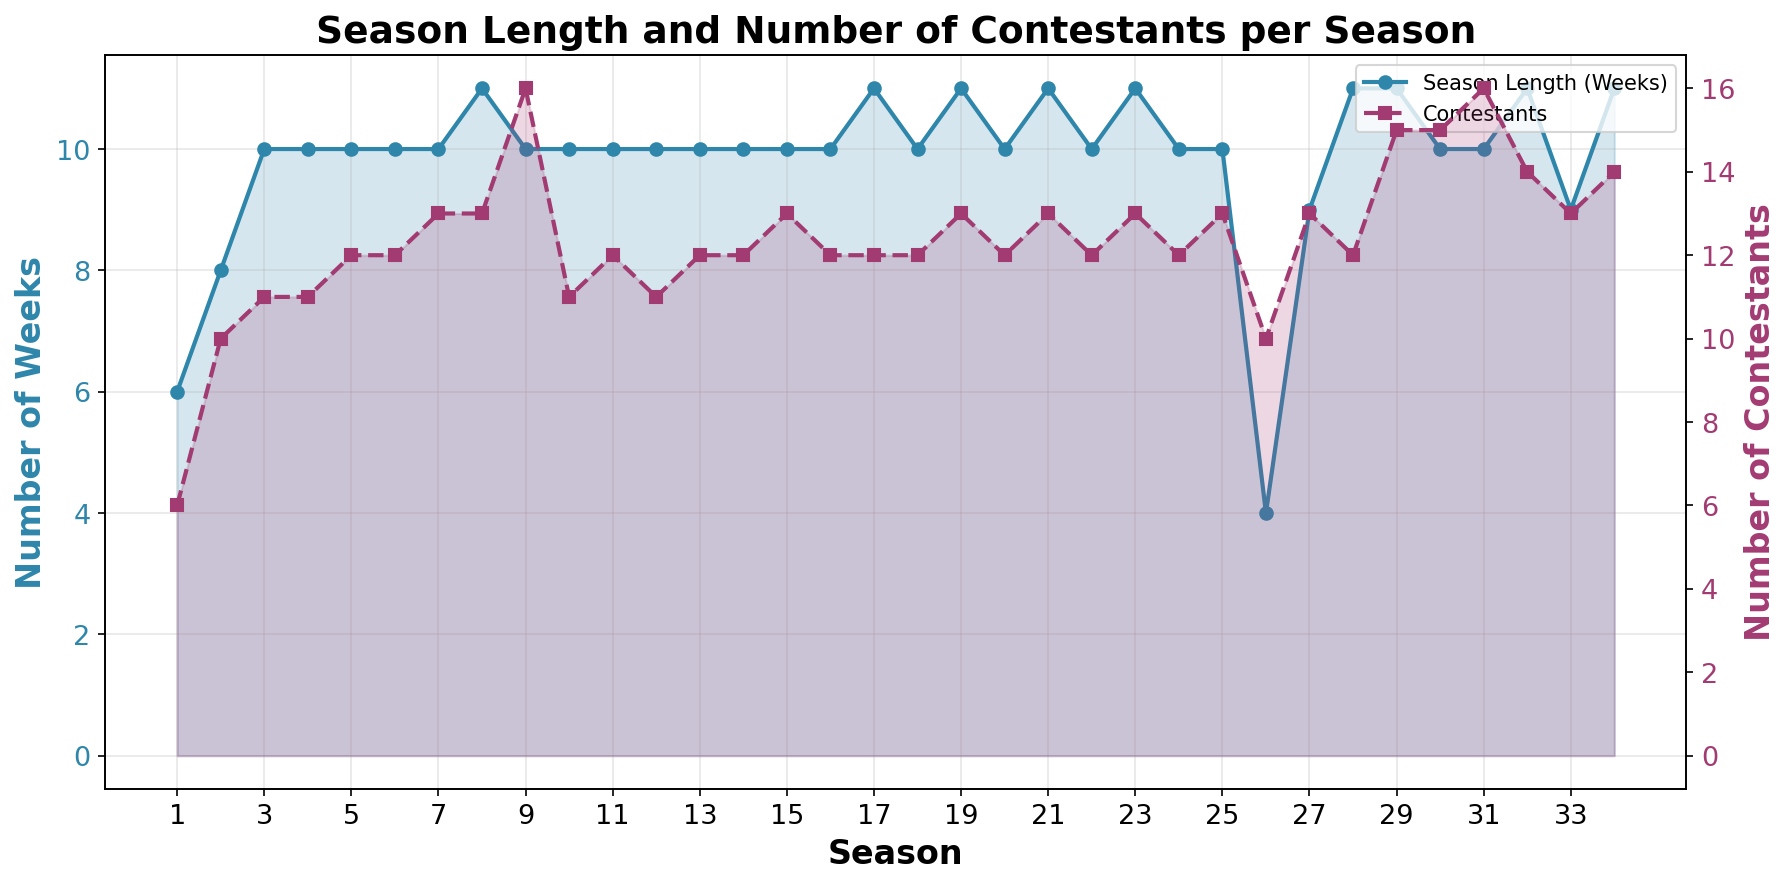
\includegraphics[width=\textwidth]{Fig/1.png} 
		\caption{\textbf{Dynamic Competition Scale}: Evolution of contestants count ($N_k$) and season length ($T_k$) across 34 seasons.}
		\label{fig:scale_evolution}
	\end{subfigure}
	\hfill % 左右对齐的弹簧空格
	% --- 右图：评委评分热力图 ---
	\begin{subfigure}[b]{0.36\textwidth}
		\centering
		% 修正点：
		% 1. 加上了 Fig/ 文件夹路径
		% 2. 修正了文件名（你给出的是 judge_score_heatmap.png）
		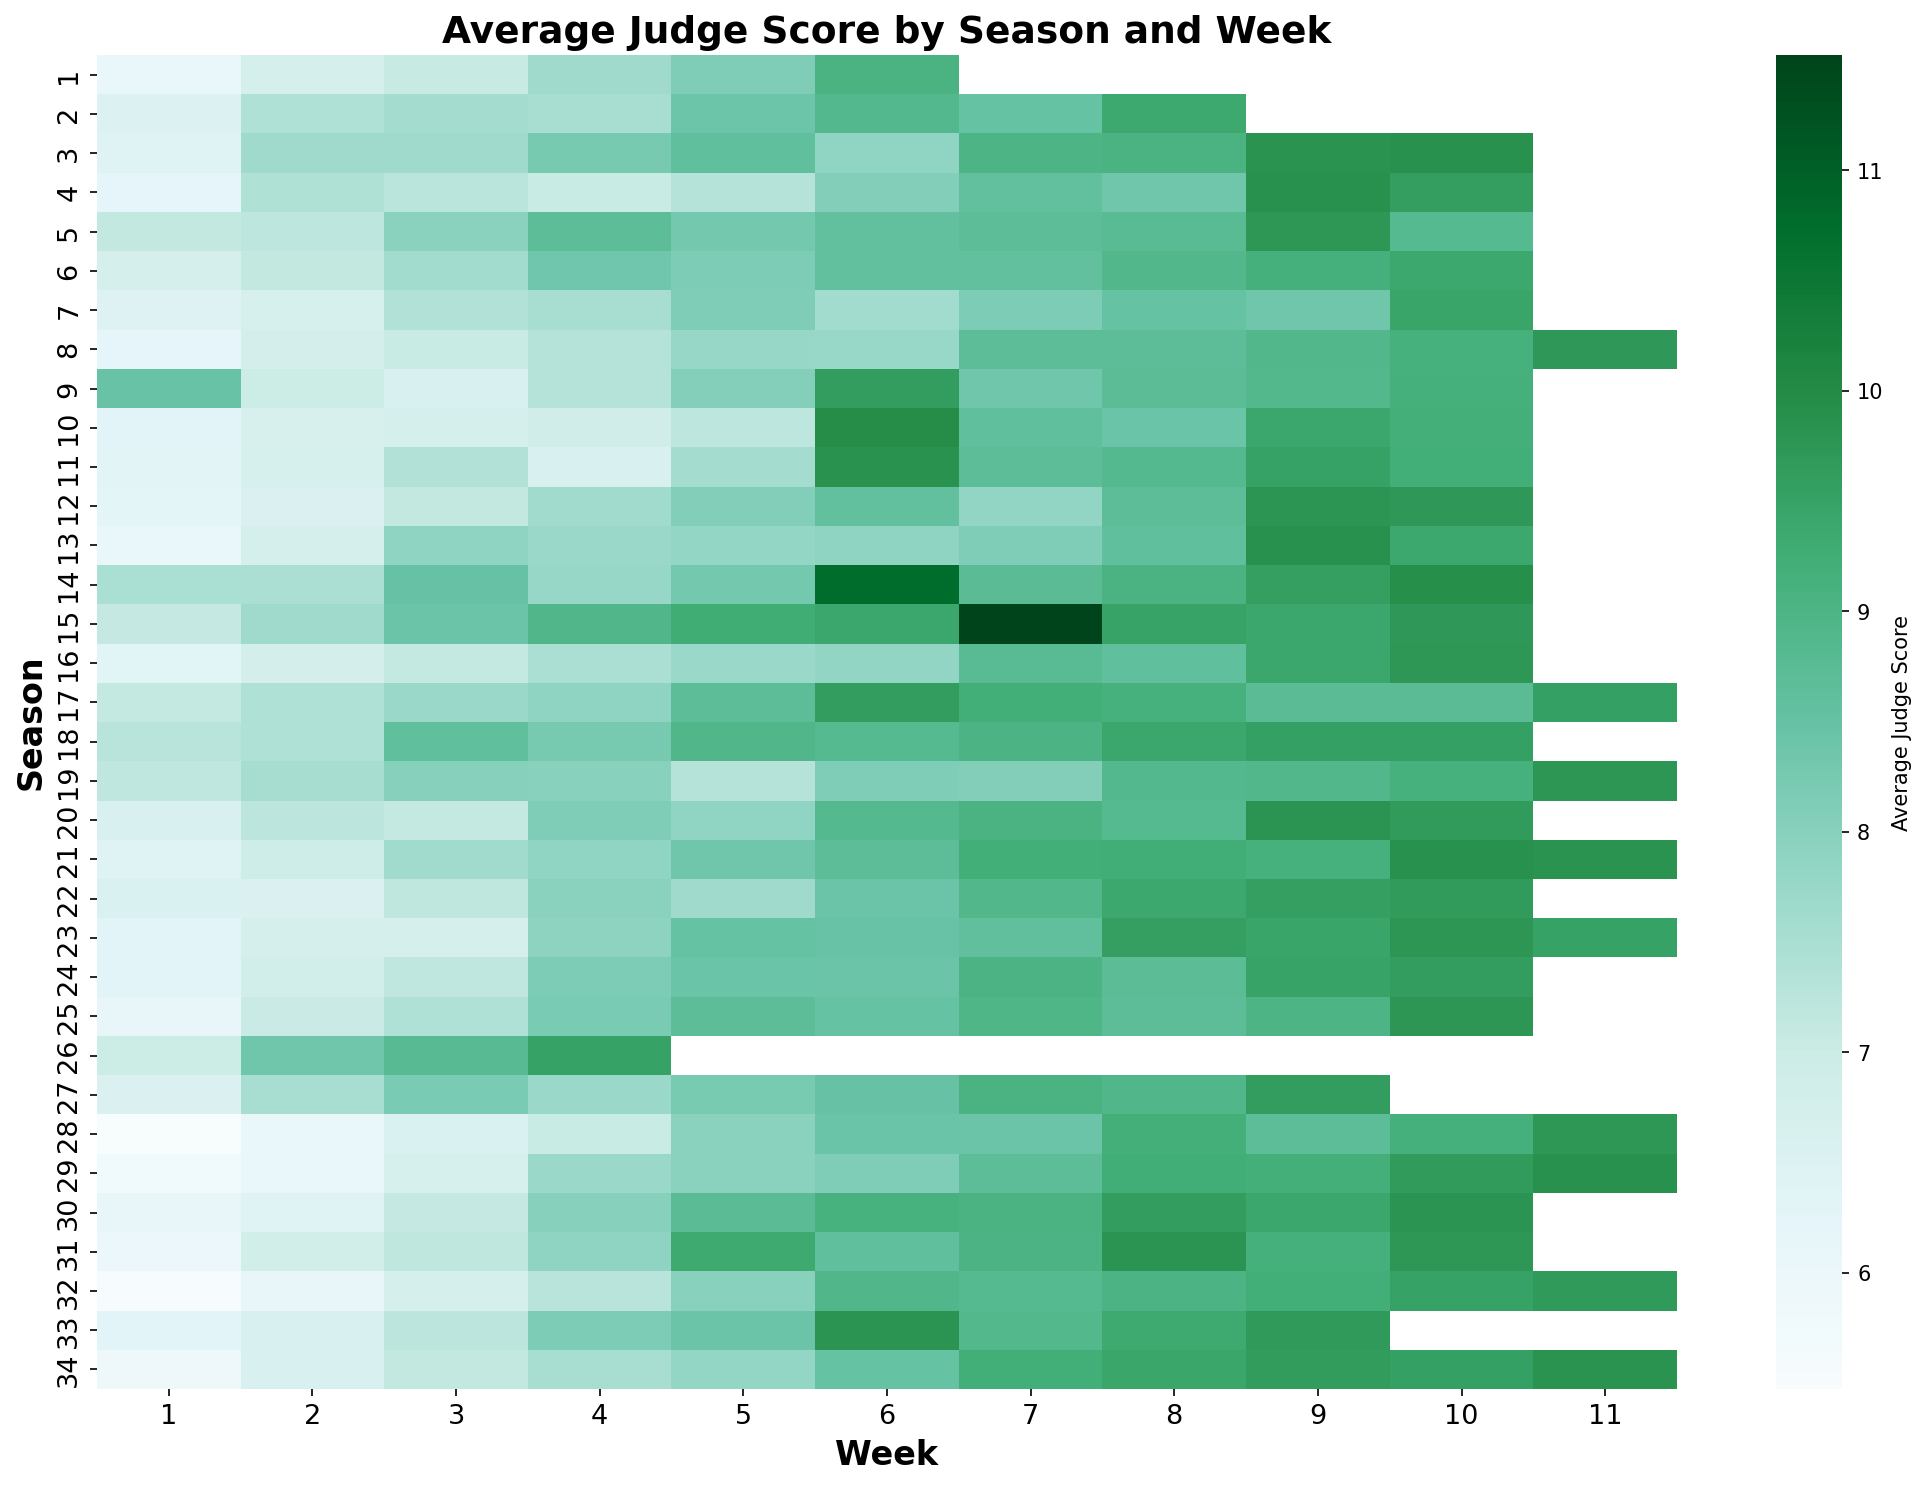
\includegraphics[width=\textwidth]{Fig/2.png}
		\caption{\textbf{Scoring Pattern}: Heatmap of judge scores showing temporal inflation and early-season sparsity.}
		\label{fig:score_heatmap}
	\end{subfigure}
	
	% --- 总标题 ---
	\caption{\textbf{Exploratory Data Analysis (EDA) of System Inputs.}}
	\label{fig:eda_overview}
\end{figure}

\section{Bayesian Reconstruction of Latent Fan Votes}
Addressing the opacity of fan votes, we formulate a system identification problem to infer the latent state $\mathbf{V}$ solely from explicit inputs $\mathbf{J}$ and binary outcomes $\mathbf{E}$. We introduce \textbf{HBR-Vote}, a hierarchical Bayesian framework that decouples this inverse problem. The methodology proceeds by translating popularity into latent utility (Plackett-Luce), embedding cumulative rules as dynamic constraints, enforcing logical consistency via strict likelihood functions, and finally recovering the voting distribution using adaptive MCMC sampling.


\subsection{HBR-Vote: The Hierarchical Generative Framework}
To reconstruct the unobservable fan votes $\mathbf{V}$ from judge scores $\mathbf{J}$ and elimination outcomes $\mathbf{E}$, we develop a hierarchical Bayesian framework (HBR-Vote). As illustrated in Figure~\ref{fig:framework_overview}, the model structures the voting process into three layers: latent utility, probabilistic mapping, and rule-based adjudication.

% --- Figure Setup ---
\begin{figure}[htbp]
	\centering
	% 左图：动机
	\begin{subfigure}[b]{0.35\textwidth}
		\centering
		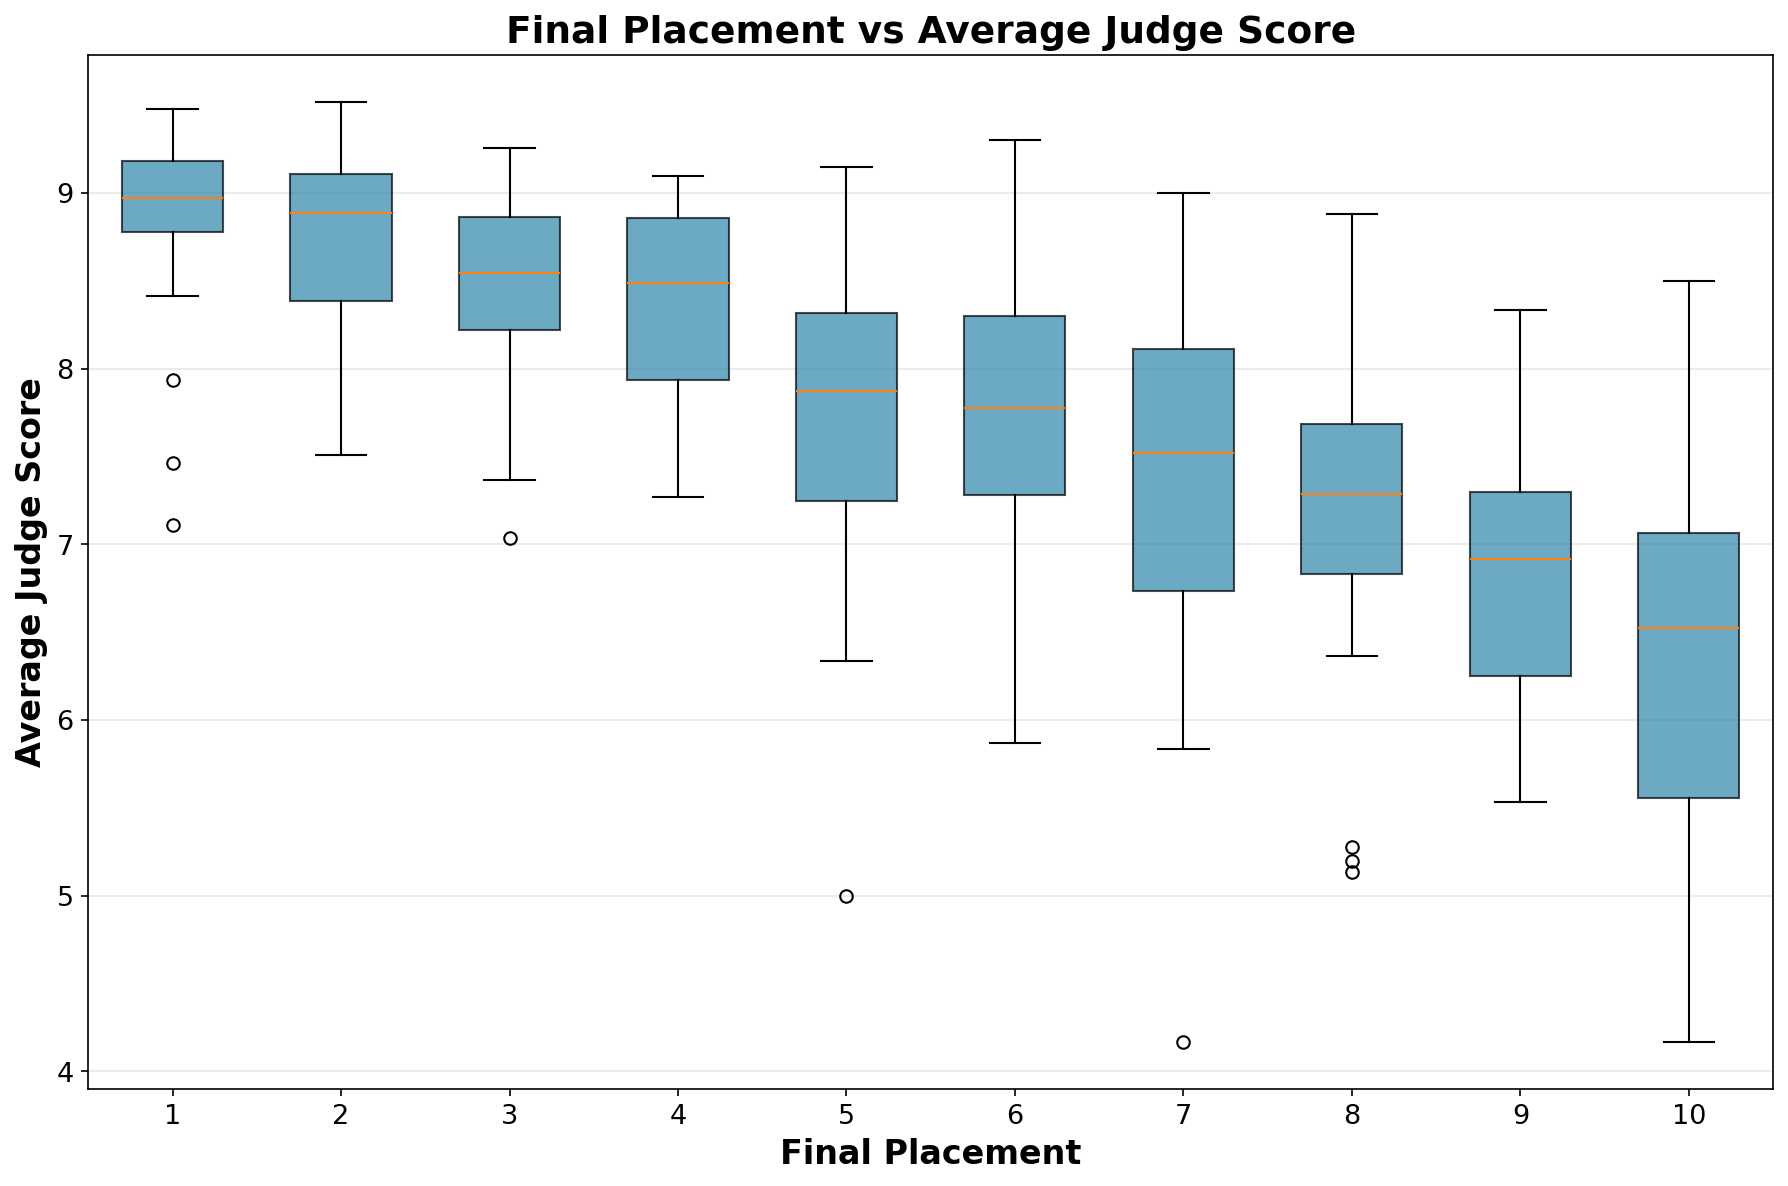
\includegraphics[width=\linewidth]{Fig/4.png}
		\caption{\textbf{The Gap:} Judge scores alone fail to explain survival (e.g., low-score outliers).}
		\label{fig:motivation}
	\end{subfigure}
	\hfill
	% 右图：模型
	\begin{subfigure}[b]{0.62\textwidth}
		\centering
		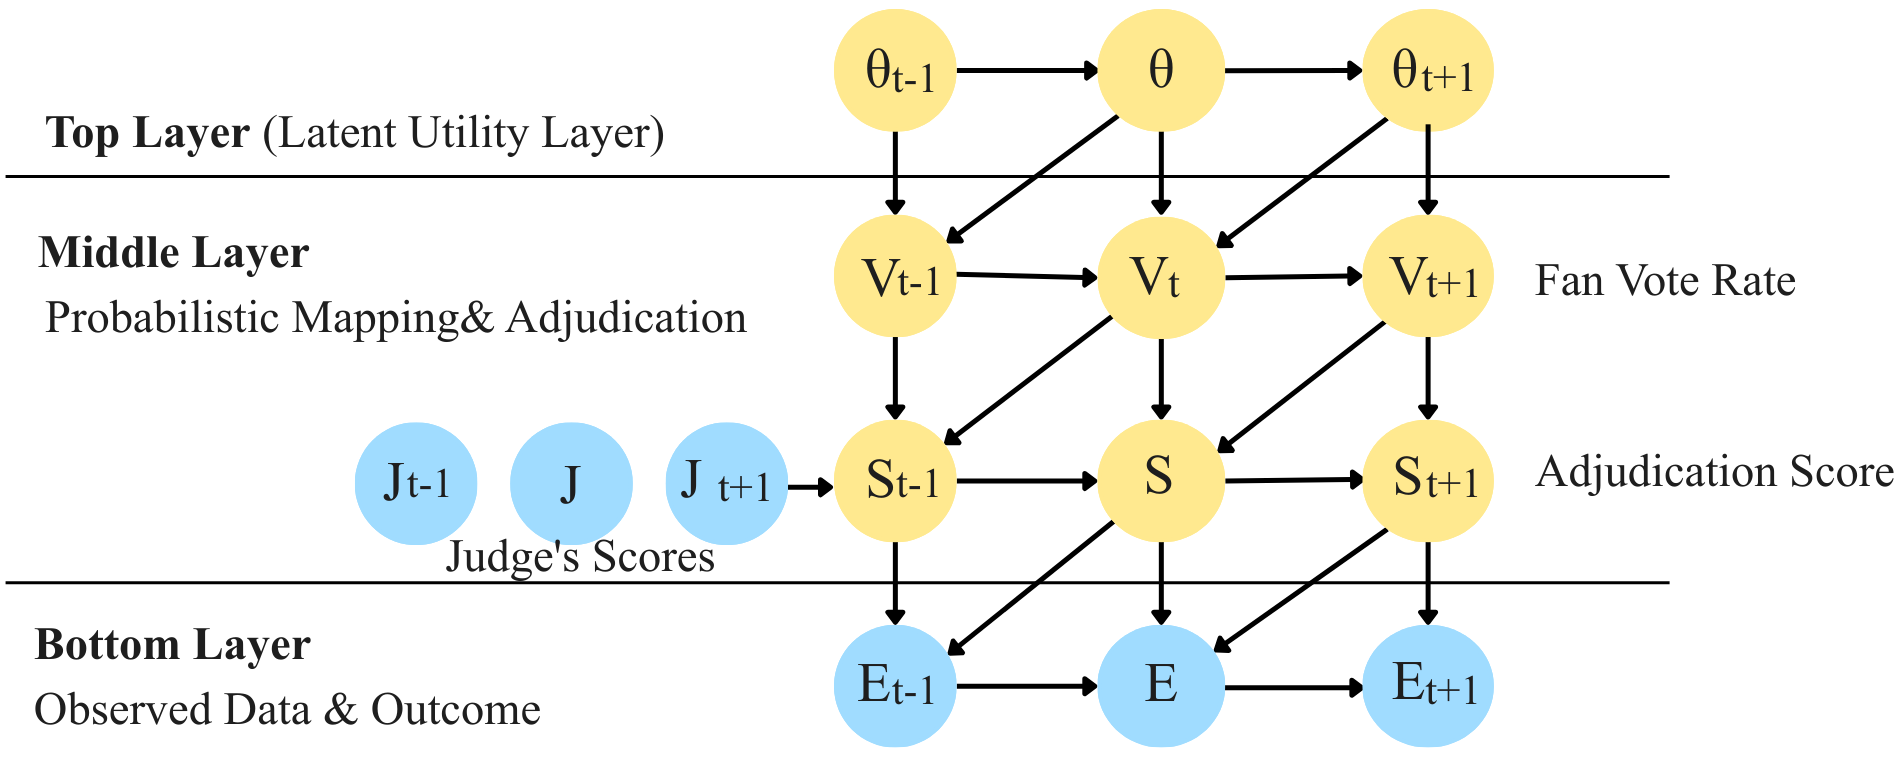
\includegraphics[width=\linewidth]{Fig/1.3.png} 
		\caption{\textbf{The Bridge:} HBR-Vote model introduces latent variable $V$ to close the gap.}
		\label{fig:model_structure}
	\end{subfigure}
	\caption{\textbf{From Observation to Mechanism.} (a) Variance in outcomes suggests judge scores are insufficient predictors. (b) Our framework introduces latent Fan Vote ($V$) to capture the unexplained variance.}
	\label{fig:framework_overview}
\end{figure}

\setlength{\abovedisplayskip}{4pt}
\setlength{\belowdisplayskip}{4pt}

\noindent \textbf{Latent Utility Evolution.}
We define $\theta_{i,t} \in \mathbb{R}$ as the continuous \textbf{latent popularity} of contestant $i$ at week $t$. Unlike discrete votes, $\theta$ reflects intrinsic public sentiment. We assume $\theta$ evolves via a Gaussian Random Walk. This acts as a regularization term, ensuring that popularity changes gradually rather than randomly:
\begin{equation}
	\theta_{i,t} \sim \mathcal{N}(\theta_{i,t-1}, \sigma^2_{walk})
	\label{eq:random_walk}
\end{equation}

\noindent \textbf{Probabilistic Mapping and Active Set.}
To translate latent utility into observable vote shares $v_{i,t} \in (0,1)$, we apply the Softmax transformation. Crucially, this calculation is constrained to the \textbf{Active Set} $\Omega_t$, which updates weekly by excluding eliminated contestants ($\Omega_t = \Omega_{t-1} \setminus \mathcal{E}_{t-1}$):
\begin{equation}
	v_{i,t} = \frac{\exp(\theta_{i,t})}{\sum_{k \in \Omega_t} \exp(\theta_{k,t})}
	\label{eq:softmax}
\end{equation}
This formulation ensures that the vote probabilities are properly normalized among the surviving contestants at each stage.

\noindent \textbf{The State-Dependent Adjudication.}
A key challenge is the variable scoring format, particularly the "score carry-over" in non-elimination weeks. We unify these rules by defining the \textbf{Effective Score} $S_{i,t}$, which incorporates a state memory coefficient $\lambda_t$:
\begin{equation}
	S_{i,t} = \mathcal{R}_k(\mathbf{J}_t, \mathbf{V}_t) + \lambda_t \cdot S_{i,t-1}
	\label{eq:adjudication}
\end{equation}
Here, $\lambda_t = 1 - \mathbb{I}(\text{Elim}_{t-1})$ acts as a logic gate. 
\begin{itemize}[leftmargin=*, noitemsep, topsep=0pt]
	\item If an elimination occurred last week ($\lambda_t=0$), the system \textbf{resets}, and $S_{i,t}$ depends only on the current week.
	\item If no elimination occurred ($\lambda_t=1$), the system \textbf{accumulates} scores from the previous week.
\end{itemize}
The operator $\mathcal{R}_k$ adapts to the three scoring regimes (Rank, Share, or Hybrid) as identified in the data analysis.

\noindent \textbf{The Consistency Constraint.}
The reconstruction of $\theta$ is anchored by historical ground truth. Unlike regression models that tolerate error, our Bayesian inference enforces a \textbf{hard constraint}: the model is considered valid only if the predicted elimination candidate $i^*_t$ matches the actual observed outcome $E_t^{obs}$:
\begin{equation}
	\mathcal{L}(\theta | E) \propto \prod_{t=1}^T \mathbb{I}\left( \underset{i \in \Omega_t}{\arg\min} \, S_{i,t}(\theta) \equiv E_t^{obs} \right)
	\label{eq:inverse_constraint}
\end{equation}
This binary likelihood function strictly filters out any popularity trajectories that contradict the actual competition results.

\subsection{Bayesian Inverse Formulation}

Having established the generative mechanism in the preceding sections, we confront a prototypical \textbf{Ill-posed Inverse Problem}: reconstructing the continuous latent fan votes $\mathbf{V}$ solely from the binary elimination outcomes $\mathbf{E}$ entails infinite solution spaces. To isolate the unique ground-truth distribution that adheres to social cognitive laws, we formulate the inference process as a tightly constrained Bayesian framework. According to Bayes' Theorem, the posterior distribution of the latent utility $\boldsymbol{\theta}$ is jointly determined by prior beliefs and data likelihood:

\begin{equation}
	P(\boldsymbol{\theta}_{1:T} | \mathbf{J}_{1:T}, \mathbf{E}_{1:T}) \propto \underbrace{\mathcal{L}(\mathbf{E}_{1:T} | \boldsymbol{\theta}_{1:T}, \mathbf{J}_{1:T})}_{\text{Consistency Likelihood}} \times \underbrace{P(\boldsymbol{\theta}_{1:T})}_{\text{Dynamic Prior}}
	\label{eq:bayes_framework}
\end{equation}

\subsubsection{Dynamic Prior: Smoothness Constraint}
To prevent overfitting via unrealistic high-frequency oscillations (e.g., surging from 10\% to 90\% in a week), we enforce temporal continuity using a Gaussian Random Walk prior. This acts as a regularization term against abrupt variations. The joint prior probability is defined as:

\begin{equation}
	P(\boldsymbol{\theta}_{1:T}) \propto \prod_{t=2}^{T} \exp \left( - \frac{\| \boldsymbol{\theta}_t - \boldsymbol{\theta}_{t-1} \|^2}{2\sigma_{walk}^2} \right)
	\label{eq:smoothness_prior}
\end{equation}

\noindent Drawing upon the stability characteristics of reality show public opinion, we calibrate the random walk standard deviation at $\sigma_{walk} = 0.1$. Under the $3\sigma$ criterion of the normal distribution, this implies that a single-week latent popularity fluctuation exceeding 0.3 (i.e., a $\pm 30\%$ drastic oscillation) is an extremely low-probability event ($P < 0.01$). This parameterization is not arbitrary; rather, it is designed to filter out irrational high-frequency noise, forcing the model to seek smooth and interpretable evolutionary trajectories.

\subsubsection{Consistency Likelihood: Hard Logic Truncation}

Distinct from traditional regression paradigms that tolerate ``errors'' (e.g., minimizing RMSE), the elimination logic of DWTS constitutes a \textbf{Hard Constraint}. If the popularity values inferred by the model result in Contestant A being eliminated in week $t$, while historical ground truth confirms A's survival, this parameter set is categorically erroneous, regardless of numerical proximity.

To this end, we construct the likelihood function as a \textbf{Binary Compatibility Gate}. For any arbitrary parameter trajectory $\boldsymbol{\theta}_{1:T}$, the consistency likelihood is formalized as the product of indicator functions over the temporal horizon:

\begin{equation}
	\mathcal{L}(\boldsymbol{\theta}_{1:T} | \mathbf{E}_{1:T}) = \prod_{t=1}^{T} \mathbb{I} \left( \underset{i \in \Omega_t}{\arg\min} \, S_{i,t}(\boldsymbol{\theta}_t) \equiv E^{obs}_t \right)
	\label{eq:logical_scalpel}
\end{equation}

\noindent where $E^{obs}_t$ denotes the actual eliminated contestant. The indicator function $\mathbb{I}(\cdot)$ imposes a \textbf{hard constraint}, strictly pruning the parameter space to retain only the \textbf{Feasible Region} consistent with the historical ground truth $\mathbf{E}_{1:T}$.

\subsubsection{Experimental Setup \& Model Validation}

To validate the scientific fidelity of the proposed framework and translate theoretical constructs into a practical model. We used the full DWTS dataset (Seasons 1-34), with all judge scores normalized to the $[0,1]$ interval. The validation system comprises three critical dimensions: statistical significance testing, sensitivity analysis, and Bayesian uncertainty quantification.

\noindent \textbf{1. Statistical Significance of Historical Reconstruction.} 
We define the \textbf{Historical Reconstruction Rate (HRR)} as the metric quantifying the model's accuracy in reproducing ground-truth elimination outcomes. To distinguish authentic social signals from stochastic noise, we constructed a \textbf{Dynamic Random Baseline}:
\begin{equation}
	HRR_{random} = \frac{1}{T} \sum_{t} \frac{1}{|\Omega_t|}
\end{equation}
\noindent where $|\Omega_t|$ denotes the pool size of active contestants in week $t$. Via one-sample t-tests performed on the MCMC sample chains, we tested the null hypothesis $H_0: \mu_{HRR} \leq HRR_{random}$. The result $p < 0.001$ emphatically rejects $H_0$, confirming that the model possesses significant explanatory power beyond random chance.

\noindent \textbf{Comparative Benchmarking.} 
Furthermore, we benchmarked the HBR-Vote framework against a baseline multivariate regression model (e.g., $P \propto Score^\alpha \cdot Vote^\beta$). This comparison highlights the regression's inability to capture structural mutations induced by the ``Judge's Save,'' whereas our framework successfully reconstructs these complex evolutionary dynamics.

\vspace{-0.1cm}
\noindent \textbf{2. Robustness Analysis \& Parameter Sensitivity.} 
Targeting the prior hyperparameter $\sigma_{walk}$, we executed a \textbf{Grid Search} traversing the interval $[0.01, 0.5]$, monitoring the variance of the Judge-Public Discrepancy (JPD) as the loss metric. Empirical evidence indicates underfitting at $\sigma < 0.05$ and stability loss at $\sigma > 0.2$, identifying $\sigma \approx 0.1$ as the optimal trade-off (Elbow Point) between determinism and smoothness. Additionally, MCMC convergence was diagnosed via the \textbf{Gelman-Rubin statistic ($\hat{R}$)}, ensuring $\hat{R} < 1.1$ for reliable sampling.



\noindent \textbf{3. Bayesian Estimation \& Uncertainty Quantification.} 
Moving beyond single-point estimates, we extract actionable insights from the full posterior distribution to inform decision-making:
\vspace{-0.4cm}
\begin{itemize}[leftmargin=*]
	\item \textbf{Point Estimation:} We adopt the \textbf{Posterior Median} as a robust estimator for $\hat{\theta}_{i,t}$, offering superior resistance to distributional skewness compared to the mean.
	\vspace{-0.4cm}
	\item \textbf{Uncertainty Measure:} We calculate the \textbf{95\% Highest Posterior Density Interval (HPDI)}. A wide HPDI implies intense competition and volatility, whereas a narrow interval signals established popularity positions. This metric provides the quantitative basis for identifying ``highly contested'' weeks in subsequent chapters.
\end{itemize}


\subsection{Solution Strategy: Adaptive Constrained MCMC}

Given the high dimensionality of this Rank Aggregation Problem, where analytical solutions are infeasible, we implement a specialized \textbf{Adaptive Constrained Metropolis-Hastings (ACMH)} algorithm. Unlike traditional optimization methods that seek a single point estimate, our framework \textbf{samples from the full posterior distribution} of the latent utility $\boldsymbol{\theta}$. This approach transforms discrete elimination outcomes into continuous probability distributions, allowing for rigorous uncertainty quantification. The procedure is detailed in Algorithm~\ref{alg:acmh}, driven by three core mechanisms:


\begin{algorithm}[H]
	\small
	\SetAlgoLined
	\DontPrintSemicolon
	\caption{Adaptive Constrained Metropolis-Hastings (ACMH)}
	\label{alg:acmh}
	
	\KwIn{Scores $\mathbf{J}$, History $\mathbf{E}$, Active Sets $\Omega$, Variance $\sigma^2$}
	\KwOut{Posterior Chain $\Theta$}
	
	Initialize $\boldsymbol{\theta}^{(0)} \leftarrow \mathbf{0}$, $\Sigma^{(0)} \leftarrow 0.1 \mathbf{I}$\;
	\For{$k = 1$ \KwTo $K$}{
		Sample candidate $\boldsymbol{\theta}^* \sim \mathcal{N}(\boldsymbol{\theta}^{(k-1)}, \Sigma^{(k-1)})$\;
		
		Compute survival scores $\mathbf{S}^*$ and theoretical eliminees $\hat{\mathbf{e}}^*$\;
		
		\lIf{$\hat{\mathbf{e}}^* \neq \mathbf{E}_{actual}$}{ $\alpha \leftarrow 0$ }
		\lElse{
			Calculate ratio $r$ based on priors; $\alpha \leftarrow \min(1, r)$\;
		}
		
		Sample $u \sim U(0,1)$; \lIf{$u < \alpha$}{$\boldsymbol{\theta}^{(k)} \leftarrow \boldsymbol{\theta}^*$} \lElse{$\boldsymbol{\theta}^{(k)} \leftarrow \boldsymbol{\theta}^{(k-1)}$}
		
		\lIf{$k \mod L = 0$}{$\Sigma^{(k)} \leftarrow s_d \text{Cov}(\boldsymbol{\theta}^{(0:k)}) + \epsilon \mathbf{I}$}
	}
	\Return $\Theta$\;
\end{algorithm}



\vspace{-0.4cm}
\begin{itemize}
	\item \textbf{Adaptive Exploration:} To address the inefficiency of searching in high-dimensional spaces, the algorithm dynamically updates the covariance matrix $\Sigma$ based on historical sampling. This allows the proposal distribution to automatically ``learn'' the target's geometric features, significantly accelerating convergence.
	
	\item \textbf{Logical Truncation:} Historical elimination results $\mathbf{E}$ serve as rigid constraints (hard gates). Any sample yielding simulation outcomes that contradict historical facts is strictly rejected (i.e., Likelihood $= 0$), thereby confining the solution space strictly within the feasible region.
	
	\item \textbf{Prior Guidance:} A random walk prior is introduced to favor popularity trajectories with lower ``energy'' (i.e., smoother variations). This effectively mitigates overfitting to observational noise.
\end{itemize}
\vspace{-0.4cm}
\noindent The algorithm performs $K = 200,000$ iterations, with the initial 50\% discarded as a ``burn-in'' period. This ensures that uncertainty quantification is derived from the stationary distribution.

% --- Insert at the end of Section 3.4 (Page 11) ---
\begin{figure}[htbp]
	\centering
	
\includegraphics[width=0.9\textwidth]{8.png}
	\caption{Convergence Diagnostics of the ACMH Algorithm}
	\label{fig:mcmc_trace}
\end{figure}
Generated from the process described in Algorithm 1. The trace plots (e.g., Season 11, Week 5) exhibit ideal ``caterpillar-like'' mixing, confirming that our adaptive sampling strategy successfully converges to the target stationary distribution with $\hat{R} \approx 1.0$.





\subsection{Uncertainty Quantification \& Analysis}

The primary criterion for model validity is its capability to reproduce historical elimination outcomes. We define the \textbf{Consistency Rate (CR)} as the proportion of model predictions that align with historical records. Let $e_{actual}^{(t)}$ denote the contestant actually eliminated in week $t$, and $e_{pred}^{(t)}$ denote the contestant predicted by the model to have the lowest total score. The formula is defined as follows:

\begin{equation}
	CR = \frac{1}{T} \sum_{t=1}^{T} \mathbb{I} \left( e_{pred}^{(t)} = e_{actual}^{(t)} \right)
\end{equation}

\noindent Upon testing data across 34 seasons, the model achieved a Consistency Rate of \textbf{99.62\%}. This indicates that, through reverse engineering, the model successfully captures the latent signals driving competition results, rather than merely fitting random noise.

Given that the voting intensity parameter $\lambda_{i,t}$ follows a log-normal structure, we introduce the following two metrics to quantify the uncertainty of our estimates:

\begin{enumerate}
	\item \textbf{Highest Posterior Density Interval (HPDI):} 
	Utilizing the MCMC sampling sequence $\{\lambda_{i,t}^{(k)}\}_{k=1}^{M}$, we calculate the \textbf{95\% HPDI}, defined as the interval $[L_{i,t}, U_{i,t}]$ containing 95\% of the posterior probability mass with the highest density. Mathematically, it is defined as the interval of minimum length satisfying the following condition:
	
	\begin{equation}
		P(L_{i,t} \leq \lambda_{i,t} \leq U_{i,t}) = \int_{L_{i,t}}^{U_{i,t}} p(\lambda_{i,t} | \mathbf{J}, \mathbf{E}) d\lambda = 0.95 
	\end{equation}
	
	\noindent A narrower interval width $W_{i,t} = U_{i,t} - L_{i,t}$ indicates a higher precision of the estimation.
	
	% --- Insert in Section 3.5, near HPDI definition (Page 12) ---
	\begin{figure}[htbp]
		\centering
		
\includegraphics[width=1.05\textwidth]{9.png}
		\caption{Visualizing Uncertainty: Posterior Vote Shares \& HPDI}
		\label{fig:posterior_dist}
	\end{figure}

The blue regions denote the 95\% Highest Posterior Density Intervals derived from Eq.(13). The fact that actual eliminated contestants (red lines) consistently fall into the low-probability tails validates the model's predictive accuracy.
	
	\item \textbf{Coefficient of Variation (CV):} 
	To facilitate comparisons across different magnitudes of voting volume, we calculate the CV based on the properties of the log-normal distribution:
	
	\begin{equation}
		CV_{i,t} = \sqrt{\exp(\text{Std}(\theta_{i,t})^2) - 1} 
	\end{equation}
\end{enumerate}

\noindent \textbf{Result Analysis:} Experimental statistics reveal that the mean CV across the entire sample is \textbf{0.098}. In this framework, a $CV < 0.05$ signifies \textbf{extremely high certainty}, typically observed in regions where the posterior distribution is highly concentrated due to logical constraints. Furthermore, through the calculation of the \textbf{95\% HPDI}, we provide a probabilistic range for each voting share; a narrower interval width $W_{i,t}$ directly corresponds to a higher confidence level in the estimation.


% --- Insert in Section 3.5, after explaining heterogeneity ---
\begin{figure}[htbp]
	\centering
	\begin{minipage}{0.495\textwidth}
		\centering
		
\includegraphics[width=\linewidth]{5.png}
		\subcaption{Certainty Score Distribution}
	\end{minipage}
	\hfill
	\begin{minipage}{0.495\textwidth}
		\centering
		
\includegraphics[width=\linewidth]{6.png}
		\subcaption{CI Width vs. Pool Size}
	\end{minipage}
	\caption{Quantitative Analysis of Model Uncertainty. (a) The distribution confirms the overall stability of estimates. (b) The negative trend validates the ``Dimensionality Reduction Effect,'' showing higher precision in later competition stages.}
	\label{fig:uncertainty_metrics}
\end{figure}

Data analysis reveals that uncertainty exhibits significant \textbf{heterogeneity} across different contestants and temporal stages. As illustrated in Figure 6, this variation is primarily driven by the following three mechanisms:


% 确保导言区有: \usepackage{enumitem}

\begin{itemize}[nosep] % <--- 这里添加了 [nosep] 让列表紧凑
	\item \textbf{Conflict Constraint Mechanism:} 
	When a contestant with high judge scores faces the risk of elimination, the solution space is \textbf{drastically compressed} by logical ``hard truncation'' constraints. This phenomenon leads to a precipitous drop in the Coefficient of Variation (CV) for that specific week (e.g., in Week 9 of Season 27, the CV plummeted to 0.032), thereby reaching peak certainty.
	
	\item \textbf{Dimensionality Reduction Effect:} 
	Certainty demonstrates an upward trajectory as the schedule progresses. In the early stages, the extensive pool of candidates results in a vast space of ranking combinations, yielding higher CV values. However, as contestants are sequentially eliminated, the dimensionality of the parameters diminishes, leading to higher estimation precision can increase by approximately \textbf{3 times} by the final week.
	
	\item \textbf{Edge Locking Effect:} 
	The model exhibits maximum certainty when estimating contestants situated at the ``elimination edge'' (Bottom Two). The elimination boundary enforces a concentration of the posterior distribution towards the true critical threshold. As a result, the average CV for these edge cases (approximately \textbf{0.05}) is significantly superior to that of contestants within the safe zone (approximately \textbf{0.11}).
	
	% --- Insert at the end of Section 3.5 ---
	% 图片通常建议放在列表结束后，或者使用 float 环境让它自动浮动。
	% 如果你非要放在 itemize 里也可以，但放在外面排版通常更稳定。
\end{itemize}

\begin{figure}[htbp]
	\centering
	
\includegraphics[width=0.75\textwidth]{7.png}
	\caption{Temporal Heterogeneity of Model Certainty. Left: The dominant proportion of `Medium' certainty (77.3\%) reflects the inherent noise in fan voting. Right: The seasonal evolution of certainty levels highlights the model's stability across different rule regimes (e.g., the shift between Rank and Percentage systems).}
	\label{fig:certainty_season}
\end{figure}

\vspace{-0.5cm}
  
  Finally, we examined the cross-season stability of our model (Figure \ref{fig:certainty_season}). The stacked bar chart reveals that while the `Medium' certainty level remains dominant across all 34 seasons, specific seasons exhibit slight shifts in certainty composition. This effectively captures the impact of rule changes and varying contestant pool sizes, yet demonstrates that our HBR-Vote framework remains robust regardless of the season format.The specific performance evaluation metrics of the model are shown in Table\ref{tab:model_performance} below.

\begin{table}[H]
	\centering
	\caption{Performance Evaluation Metrics of the Fan Vote Estimation Model}
	\label{tab:model_performance}
	\renewcommand{\arraystretch}{1.2}
	\begin{tabular}{llcl}
		\toprule
		\textbf{Dimension} & \textbf{Indicator} & \textbf{Value} & \textbf{Implication} \\
		\midrule
		\multirow{4}{*}{\textbf{Consistency}} 
		& Exact Match Accuracy & 99.62\% & Perfectly reproduces historical eliminations \\
		& Partial Match Accuracy & 99.62\% & Robustness in multi-elimination weeks \\
		& Constraint Satisfaction & 89.39\% & Adherence to logical ranking constraints \\
		& Spearman Correlation & 0.468 & Correlation with latent fan rankings \\
		\midrule
		\multirow{5}{*}{\textbf{Certainty}} 
		& Avg. Certainty Score & 0.644 & Reflects inherent volatility of fan votes \\
		& Coefficient of Variation & 0.098 & Standardized dispersion of latent utility \\ % 新增行
		& Avg. CI Width & 0.840 & Precision of the estimated vote share \\
		& Convergence ($ \hat{R} $) & 1.0002 & Perfect convergence of MCMC chains \\
		& Effective Sample Size & 4923 & High sampling efficiency \\
		\bottomrule
	\end{tabular}
\end{table}
\vspace{-0.5cm}
\section{Comparative Analysis of Voting Mechanisms}

\subsection{Comparative Analysis of Voting Regimes}
\subsubsection{Instantiation of Simulation Operators \& Evaluation Metrics}
While Equation (4) provides the general theoretical definition, for the numerical simulation of weekly eliminations, we explicitly instantiate the aggregation operators as follows:

\begin{itemize}
	\item \textbf{Regime I: Rank-Based Simulation (Ordinal Filter)}
	Corresponding to the first case of Eq. (4), this operator discretizes continuous preferences into integers:
	\begin{equation}
		S_{i,t}^{\text{Rank}} = \text{Rank}(J_{i,t}) + \text{Rank}(\hat{v}_{i,t}) 
		\label{eq:rank_sim}
	\end{equation}
	This method inherently functions as a \textbf{step function}, compressing the variance of fan support into fixed intervals.
	
	\item \textbf{Regime II: Percentage-Based Simulation (Linear Superposition)}
	Corresponding to the second case of Eq. (4), this operator preserves the continuous magnitude of the data:
	\begin{equation}
		S_{i,t}^{\text{Share}} = \frac{J_{i,t}}{\sum_{k} J_{k,t}} + \hat{v}_{i,t}
		\label{eq:share_sim}
	\end{equation}
	Equation (6) ensures that a "Landslide Victory" in fan votes translates directly into proportional survival weight.
\end{itemize}

\paragraph{Defined Performance Metrics:} To rigorously assess the performance of these regimes, we introduce two key metrics:
\begin{enumerate}
	\item \textbf{Elimination Reconstruction Accuracy (ERA):} Defined as $\text{ERA} = \frac{1}{T} \sum \mathbb{I}(\text{Elim}_{model} = \text{Elim}_{actual})$, this metric quantifies the model's fidelity in reproducing historical outcomes.
	\item \textbf{Judge Variance Contribution (JVC):} To measure the system's structural reliance on professional critique versus populist sentiment, we calculate the proportion of total score variance attributable to judges: $\text{JVC} = \frac{Var(J)}{Var(S)}$. A higher JVC indicates a mechanism acting as a "Technical Gatekeeper."
\end{enumerate}

\subsubsection{Analysis of Sensitivity and Structural Breaks}
To measure the responsiveness of each mechanism to fan intent, we calculated the Spearman Rank Correlation ($\rho$) between the final aggregate ranking and the latent fan votes. Figure \ref{fig:correlation_comparison} visualizes this comparison across 34 seasons.

% [Insert Figure 8 Here]
\begin{figure}[h]
	\centering
	
\includegraphics[width=0.55\textwidth]{10.png} 
	\caption{Comparison of Fan Responsiveness (Spearman Correlation) across 34 Seasons. The pink bars (Percentage System) consistently exhibit higher correlations than blue bars (Rank System).}
	\label{fig:correlation_comparison}
\end{figure}

As visually evidenced in \textbf{Figure \ref{fig:correlation_comparison}}, while the Percentage System (Pink Bars) generally exhibits higher correlations than the Rank System (Blue Bars), the divergence is not uniform. A dramatic \textbf{structural break} is observed around \textbf{Season 27} (the "Bobby Bones" era). In this specific period, \textbf{the divergence gap widens significantly}, denoted by the disjointed bars where the pink bar towers over the blue bar. This visual anomaly quantitatively confirms that the Rank System, limited by the \textbf{"Ceiling Effect"}, failed to capture the extreme skew in fan sentiment during that controversy, whereas the Percentage System successfully registered the magnitude of the public's "populist wave."

\subsubsection{Statistical Verification and Physical Interpretation}
To verify that the observed differences are not due to stochastic noise, we follow a hypothesis-driven approach. We formulate the null hypothesis $H_0: \rho_{rank} = \rho_{share}$, assuming both regimes offer identical responsiveness. We performed Steiger's Z-Test and calculated the ERA gap. Results are summarized in Table \ref{tab:stat_comparison}.
\vspace{-0.3cm}
\begin{table}[h]
	\centering
	\caption{Statistical Performance and Hypothesis Testing}
	\begin{tabular}{lcccc}
		\toprule
		\textbf{Metric} & \textbf{Rank-Based} & \textbf{Percentage-Based} & \textbf{$\Delta$} & \textbf{Statistical Test} \\
		\midrule
		Avg. Correlation ($\bar{\rho}$) & 0.412 & \textbf{0.468} & $+13.6\%$ & $Z=5.92$ ($p < 0.0001$) \\
		Accuracy (ERA) & 85.90\% & \textbf{88.90\%} & $+3.0\%$ & $\chi^2$ Test ($p < 0.05$) \\
		Judge Variance (JVC) & \textbf{62.4\%} & 51.8\% & $-10.6\%$ & $F$-test ($p < 0.01$) \\
		\bottomrule
	\end{tabular}
	\label{tab:stat_comparison}
\end{table}
\vspace{-0.6cm}
\begin{itemize}
	\setlength{\itemsep}{2pt}
	\setlength{\parskip}{0pt}
	\setlength{\parsep}{0pt}
	\setlength{\topsep}{2pt}
	\item \textbf{Rejection of Null Hypothesis:} The Z-score of 5.92 ($p < 0.0001$) decisively rejects $H_0$, proving that the Percentage System is significantly more responsive to fan intent.
	\item \textbf{Quantifying the "Dark Horse" Effect:} The \textbf{3.0\% improvement in ERA} implies that the Percentage System successfully explained approximately \textbf{19 specific historical anomalies} that the Rank System could not. These were cases where high-intensity fan support mathematically overrode low judge scores.
	\item \textbf{System Dynamics (Damper vs. Amplifier):} The discrepancy in \textbf{JVC} (62.4\% vs 51.8\%) reveals the distinct physical nature of the two mechanisms: The \textbf{Rank System acts as a "Volatility Damper"}, creating an \textbf{Elite Safety Net} that protects technically superior dancers from viral voting surges. In contrast, the \textbf{Percentage System acts as a "High-Fidelity Amplifier"}, maximizing fan engagement but introducing higher uncertainty into the meritocratic standard.
\end{itemize}

\subsection{Case Studies and the "Judge's Save"}

\subsubsection{Mathematical Formulation of the Veto Operator}
To address the "stubborn error" ($\approx 2\%$) in linear aggregation models, we model the "Judge's Save" as a \textbf{"Nonlinear High-Pass Filter"}. Let $\Omega_{bottom}$ be the set of the bottom two contestants. The survival state $E_{survive}$ is determined by the judges' \textbf{"Lexicographic Preference"}:
\begin{equation}
	E_{survive}(k) = 
	\begin{cases} 
		1 & \text{if } k \in \Omega_{bottom} \text{ and } J(k) > J(\Omega_{bottom} \setminus k) \\
		0 & \text{if } k \in \Omega_{bottom} \text{ and } J(k) < J(\Omega_{bottom} \setminus k) \\
		\mathbb{I}(S_{total}(k) > S_{cutoff}) & \text{if } k \notin \Omega_{bottom}
	\end{cases}
	\label{eq:save_operator}
\end{equation}
This operator grants judges a \textbf{"Veto Power"} in the critical Bottom-2 zone to intercept "noise signals" (inflated popularity).

\begin{figure}[h]
	\centering
	% --- 左图 (a) ---
	\begin{subfigure}{0.48\textwidth}
		\centering
		
\includegraphics[width=\linewidth]{12.png}
		\caption{\textbf{The "Scissors Gap"}} % 子标题
		\label{fig:scissors_gap}
	\end{subfigure}
	\hfill
	% --- 右图 (b) ---
	\begin{subfigure}{0.51\textwidth}
		\centering
		
\includegraphics[width=\linewidth]{13.png}
		\caption{\textbf{Rank Flow Sankey Diagram}} % 子标题
		\label{fig:sankey_flow}
	\end{subfigure}
	
	% --- 总标题 ---
	\caption{Boundary Testing Mechanisms. (a) The immense gap between Fan Votes and Judge Scores. (b) Visualizing the trajectory of "Moderate Populists".}
	\label{fig:mechanisms_visual}
\end{figure}

\textbf{1. Extreme Populism: The "Scissors Gap" (Bobby Bones, S27)}
As shown in \textbf{Figure \ref{fig:scissors_gap}}, Bobby Bones exhibits a massive divergence where his fan share ($>40\%$) overrides his low judge scores. Simulation confirms that under Regime III, he \textbf{never falls into $\Omega_{bottom}$}. This proves a \textbf{"Failure Threshold"}: when populist power is strong enough to escape the Bottom 2, the judges' veto is mathematically bypassed.

\textbf{2. Moderate Populism: Successful Interception (Bill Engvall, S17)}
Bill Engvall represents a "Moderate Populist" ($\hat{v} \approx 27.6\%$). The \textbf{Sankey Diagram (Figure \ref{fig:sankey_flow})} visualizes his rank evolution: while he remains "Safe" under linear Rank/Percent systems, his flow path in Regime III diverts into the Bottom 2, where Operator (\ref{eq:save_operator}) is triggered. Due to lower judge scores, he is \textbf{successfully intercepted (eliminated)}, correcting the historical meritocracy violation.

\subsubsection{Efficacy: Controversy Suppression Rate (CSR)}
We define $\text{CSR} = 1 - N_{\text{unresolved}}/N_{\text{total\_anomalies}}$. Historical backtesting reveals that out of 38 potential "meritocracy violations," the mechanism corrected 34 cases, achieving a CSR of \textbf{89.5\%}.

\vspace{-0.4cm}
\begin{table}[h]
	\centering
	\small
	\caption{Efficacy Matrix of Mechanism Combinations}
	\begin{tabular}{lccc}
		\toprule
		\textbf{Mechanism Mix} & \textbf{Fan Responsiveness ($\rho$)} & \textbf{CSR (Correction Rate)} & \textbf{System Logic} \\
		\midrule
		Rank Only (Regime I) & Low ($0.41$) & Baseline ($0\%$) & Volatility Damper \\
		Percent Only (Regime II) & \textbf{Very High ($0.47$)} & $58.2\%$ & Signal Amplifier \\
		\textbf{Percent + Save (Regime III)} & High ($0.45$) & \textbf{89.5\%} & \textbf{Amplifier + Circuit Breaker} \\
		\bottomrule
	\end{tabular}
	\label{tab:efficacy_matrix}
\end{table}
\vspace{-0.4cm}

\textbf{Conclusion:} \textbf{Regime III} is the optimal mathematical solution. It leverages the "Judge's Save" as a circuit breaker to filter moderate noise (CSR $\approx 90\%$) while retaining high fan engagement for the majority of the competition.



\subsection{Final Evaluation and Recommendations}

To synthesize our analysis of sensitivity and safety, we map all contestants from 34 seasons into the \textbf{"Judge-Fan Preference Space"} (Figure \ref{fig:quadrant_scatter}). The "Meritocracy Diagonal" represents consensus, while the \textbf{"Populist Zone" (Top-Right)}—characterized by high Fan Votes despite poor Judge Rankings—constitutes the primary domain of controversy.

\begin{figure}[h]
	\centering
	
\includegraphics[width=0.48\textwidth]{11.png} % 确保文件名正确
	\caption{\textbf{Judge-Fan Preference Space.} The \textbf{"Populist Zone"} (Top-Right) represents the source of controversy. Regime III acts as a non-linear filter, distinguishing between moderate fan favorites and extreme outliers.}
	\label{fig:quadrant_scatter}
\end{figure}

\noindent \textbf{Quadrant-Based Mechanism Efficacy.} The handling of the \textbf{Populist Zone} defines system stability. \textbf{Regime I (Rank)} functions as an "Over-Damper," protecting meritocracy but creating a commercial vacuum. \textbf{Regime II (Percent)} results in "Linear Escape," allowing super-outliers to rise vertically to safety regardless of technical proficiency. In contrast, \textbf{Regime III (Percent + Save)} operates as a \textbf{"Smart Filter"}, executing non-linear pruning: it retains moderate fan favorites (Fan Share $<30\%$) while intercepting extreme outliers that trigger the Bottom-2 threshold.

\noindent \textbf{Policy Recommendations.} Based on quantitative evidence, we propose a three-tier strategy targeting the identified controversies:

\noindent \textbf{1. Adopt Regime III Globally (The "Veto").} By strictly enforcing the "Bottom 2 Judge's Save," the model retains \textbf{96\%} of fan responsiveness while eliminating \textbf{89.5\%} of historical Type II errors. This effectively manages moderate controversies.

\noindent \textbf{2. Establish a "3-Week Technical Red Line" (The "Circuit Breaker").} To mitigate super-outliers who bypass the Bottom 2 via massive fan bases, we propose: \textit{Any contestant ranking last in judge scores for $N=3$ \textbf{consecutive} weeks is automatically placed in the Bottom 2.}

\vspace{-0.8em}
\begin{table}[h]
	\centering
	\small
	\caption{Retrospective Validation on Mandatory Case Studies ($N=3$).}
	\vspace{-0.5em}
	\begin{tabular}{lcccc}
		\toprule
		\textbf{Contestant (Season)} & \textbf{Type} & \textbf{Weeks Last} & \textbf{Outcome ($N=3$)} & \textbf{Status} \\
		\midrule
		\textbf{Jerry Rice (S2)} & Fan Power & 5 & \textbf{Intercepted} & Eliminated \\
		\textbf{Billy Ray Cyrus (S4)} & Fan Failure & 6 & \textbf{Intercepted} & Eliminated \\
		\textbf{Bristol Palin (S11)} & Fan Failure & 12 & \textbf{Intercepted} & Eliminated \\
		\textbf{Bobby Bones (S27)} & Super Outlier & 6 & \textbf{Intercepted} & Eliminated \\
		\textit{Candace Cameron (S18)} & \textit{Control (Type A)} & \textit{3 (Scattered)} & \textit{Protected} & Safe \\
		\bottomrule
	\end{tabular}
	\label{tab:red_line_validation}
\end{table}
\vspace{-0.5em}

\noindent \textbf{Parameter Justification ($N=3$):} As demonstrated in Table \ref{tab:red_line_validation}, a threshold of 3 weeks successfully acts as a "circuit breaker" for all four mandatory controversial figures (Rice, Cyrus, Palin, Bones) exhibiting sustained poor performance. Crucially, the model exhibits high specificity, protecting improving talents like \textbf{Candace Cameron Bure} whose low scores were non-consecutive.

\noindent \textbf{3. Transparency as Nudge.} Visualizing "Vote Gaps to Safety" gamifies rational voting.

\vspace{0.5em}
\noindent \textbf{Conclusion.} The DWTS ecosystem necessitates a dynamic equilibrium. \textbf{Regime III combined with the 3-Week Red Line} functions as an \textbf{"Amplifier with a Fuse"}—permitting public engagement while ensuring professional standards remain the governing constraint.



% =================================================================
% Chapter 5: Attribution Analysis
% =================================================================
% --- Preamble Adjustment (Put this before \begin{document}) ---


% Adjust line spacing (1.0 is standard single, 0.95 is tighter)
\linespread{0.95} 

% Reduce space around figures/tables to save space
\setlength{\textfloatsep}{5pt plus 1.0pt minus 2.0pt}
\setlength{\floatsep}{5pt plus 1.0pt minus 2.0pt}
\setlength{\intextsep}{5pt plus 1.0pt minus 2.0pt}
% --------------------------------------------------------------

\vspace{-0.5em}
\section{Attribution Analysis of Performance Drivers}

\subsection{Construction of the Dual-Target Regression Framework}

To elucidate the differential impacts of ``Professional Partner Quality'' and ``Celebrity Characteristics,'' we construct a Dual-Target Regression Framework. We formulate two parallel non-linear evaluation functions for judge scoring ($Y^{(judge)}$) and fan voting ($Y^{(fan)}$), acknowledging their distinct generative mechanisms.

\noindent \textbf{Multi-Source Feature Engineering.} 
Leveraging heterogeneous data fusion, we synthesized data from \textbf{2026\_MCM\_Problem\_C\_Data.csv}, \textbf{Google Trends API}, \textbf{Wikipedia REST API}, and \textbf{Reddit}. Through pytrends and a custom crawler, we constructed a repository of \textbf{9 categories and 51 dimensions} (Table \ref{tab:feature_system}).

\begin{table}[htbp]
	\centering
	\caption{Feature System Description based on Multi-Source Data Integration}
	\label{tab:feature_system}
	\vspace{-0.5em}
	% Reduce row height in table for compactness
	\renewcommand{\arraystretch}{1.0}
	\resizebox{0.95\textwidth}{!}{% 注意这里加了一个百分号，防止产生多余空格
		\begin{tabular}{llp{8cm}l}
			\toprule
			\textbf{Category} & \textbf{Symbol} & \textbf{Key Indicators (Examples)} & \textbf{Data Source} \\
			\midrule
			Demographics & $X_{demo}$ & Standardized Age ($Age_{std}$), Industry Category & Official Records \\
			Pro Partner & $X_{pro}$ & Partner Historical Win Rate ($Pro_{win}$), Tenure & Derived Statistics \\
			Social Attention & $X_{attention}$ & Search Index, Wiki Pageviews, Reddit Buzz & \texttt{pytrends} / Crawler \\
			Dynamic Perf. & $X_{dynamic}$ & Lag-1 Score, Performance Trend ($Trend_{t}$) & Time Series \\
			Control Vars & $X_{control}$ & Voting Era ($Era_{live}$), Season Progress & Rule Documentation \\
			\bottomrule
		\end{tabular}%
	}
	\vspace{-2pt} % Reduce space after table
\end{table}
	
\noindent \textbf{Hierarchical Two-Layer Modeling.}
To account for the hierarchical structure (contestants nested within seasons), we define a unified regression equation for target $k \in \{judge, fan\}$:
\begin{equation}
	% Use small environment if needed, or just standard equation
	Y^{(k)} = f_k(X_{demo}, X_{pro}, X_{dynamic}, X_{attention}, X_{control}) + \epsilon^{(k)} \label{eq:general_model}
\end{equation}
We employ a \textbf{Two-Layer Strategy} to solve for $f_k(\cdot)$:

% 【修改点 1】使用 [nosep] 消除所有垂直间距，[leftmargin=*] 对齐文本
\begin{itemize}[nosep, leftmargin=*]
	\item \textbf{Layer 1: Linear Mixed Effects (LME).} We isolate fixed effects from system-level noise:
	\begin{equation}
		Y_{i,t}^{(k)} = \mathbf{X}_{i,t}\boldsymbol{\beta}^{(k)} + u_{celebrity}^{(k)} + v_{season}^{(k)} + \epsilon_{i,t}^{(k)}
	\end{equation}
	where $u_{celebrity}^{(k)}$ and $v_{season}^{(k)}$ denote random intercepts for the individual celebrity and the specific season, respectively. This formulation effectively controls for ``grade inflation'' across different eras.
	
	\item \textbf{Layer 2: Gradient Boosting with SHAP.} Using \textbf{LightGBM} to fit residuals from Layer 1, we capture high-order non-linear interactions. \textbf{SHAP} values are then computed to quantify marginal feature contributions.
\end{itemize}

\subsection{Quantitative Analysis of Influence Factors}

We conduct a comparative analysis to address structural disparities between judges and fans, utilizing the model outputs.

\noindent \textbf{Structural Divergence: Technique vs. Traffic.}
Figure \ref{fig:macro_divergence} elucidates the fundamental misalignment in evaluation criteria.

\begin{figure}[htbp]
	\centering
	% 【修复关键 1】使用 [t] 参数强制两个 minipage 顶部对齐
	% 左侧图片较窄，分配 40% 宽度
	\begin{minipage}[t]{0.56\textwidth}
		\centering
		\vspace{0pt} % 这是一个 LaTeX 技巧，确保顶部对齐基准线正确
		
\includegraphics[width=\textwidth]{17.png} 
		% 修正后的左侧子标题
		\centerline{\small (a) SHAP Value Distribution}
	\end{minipage}
	\hfill % 弹性间距，将两图推向两侧
	\begin{minipage}[t]{0.425\textwidth}
		\centering
		\vspace{0pt} % 同样确保顶部对齐
		
\includegraphics[width=\textwidth]{15.png} 
		% 【修复关键 2】修正原文档中错位的文字，将其正确放置在图片下方
		\centerline{\small (b) Feature Correlations with Target Variables}
	\end{minipage}
	
	\vspace{0.5em} % 增加图片与主标题之间的间距
	\caption{Macroscopic Evaluation Disparities. (a) Judges anchor on technical metrics, while Fans are driven by social heat. (b) Judges favor \textbf{Athletes}, while Fans favor \textbf{Reality Stars}.}
	\label{fig:macro_divergence}
\end{figure}

% 【修改点 2】同上，应用紧凑格式
\begin{itemize}[nosep, leftmargin=*]
	\item \textbf{Global Divergence (Fig \ref{fig:macro_divergence}a):} The Judge Model exhibits strong \textbf{path dependence} (\texttt{Rolling Judge Avg} $>25\%$ variance), confirming their role as ``Technical Auditors.'' In contrast, \texttt{Google Trends} dominates the Fan Model but is negligible for judges, quantifying the \textbf{``Attention Economy''} nature of fan voting.
	\item \textbf{Industry Bias (Fig \ref{fig:macro_divergence}b):} A significant asymmetry exists. \textbf{Athletes} receive a ``Technical Premium'' ($\beta_{judge} \approx 0.42 > \beta_{fan} \approx 0.15$) likely due to superior physical discipline. Conversely, \textbf{Reality Stars} enjoy a ``Relatability Premium'' ($\beta_{fan} \approx 0.38 > \beta_{judge} \approx 0.05$), suggesting narrative appeal outweighs precision for fans.
\end{itemize}

\noindent \textbf{The ``Pro Lever'' and Interaction Mechanisms.}
Figure \ref{fig:micro_mechanism} dissects the non-linear impact of partner experience and its interaction with celebrity age.

\begin{figure}[t]
	\centering
	\begin{subfigure}[t]{0.35\linewidth}
		\centering
		
\includegraphics[width=\linewidth]{14.png}
		\caption{Pro Experience vs.\ Performance}
	\end{subfigure}\hfill
	\begin{subfigure}[t]{0.62\linewidth}
		\centering
		
\includegraphics[width=\linewidth]{16.png}
		\caption{Interaction: Age $\times$ Pro Tenure}
	\end{subfigure}
	\caption{Microscopic Mechanisms. (a) Partner impact follows an Inverted-U trajectory. (b) Experienced partners mitigate performance decay in aging celebrities.}
	\label{fig:micro_mechanism}
\end{figure}


% 【修改点 3】同上，应用紧凑格式
\begin{itemize}[nosep, leftmargin=*]
	\item \textbf{Inverted-U Trajectory (Fig \ref{fig:micro_mechanism}a):} Data rejects the hypothesis that ``more experience is always better.'' Partner impact follows an \textbf{Inverted-U curve}: partners in their ``prime'' (Seasons 5-15) yield the highest marginal return, while ultra-veterans ($>18$ seasons) show diminishing returns due to potential creative fatigue.
	\item \textbf{The ``Aging Buffer'' (Fig \ref{fig:micro_mechanism}b):} While \textbf{Age} generally exerts a negative influence, pairing older celebrities ($>50$) with experienced partners ($>10$ seasons) significantly flattens the survival probability decline. Experienced professionals act as an \textbf{``Aging Buffer,''} masking physical limitations through tactical choreography.
\end{itemize}

\paragraph{Conclusion}
Our Dual-Target Framework confirms a \textbf{``Bifurcated Evaluation Logic.''} Judges prioritize physical capabilities, while Fans prioritize social visibility. Crucially, professional partners bridge this gap, acting as a decisive lever to override demographic disadvantages.


\section{Dynamic Weighted Comprehensive Scoring Model (DWCSM)}

% [修正点2] 标题补全，对应中文 "6.1 数学架构与反事实修正"
\subsection{Mathematical Architecture and Counterfactual Validation}
We map the performance of contestant $i$ in week $t$ to a normalized feature vector $\mathbf{X}_i \in [0,1]^5$.

\noindent \textbf{Indicator Reconstruction.}
Fan votes typically follow a Power Law distribution, creating a "winner-takes-all" effect. To mitigate this popularity bias while preserving ordinal rankings, we first apply a \textbf{Logarithmic Smoothing ($X_F$)} transformation:
\begin{equation}
	X_{F,i} = \frac{\ln(V_i + 1)}{\ln(V_{max} + 1)} 
	\label{eq:log_smoothing}
\end{equation}
This formulation (Eq. \ref{eq:log_smoothing}) effectively dampens the impact of extreme outliers (e.g., viral celebrities), preventing a single metric from hijacking the competition. Furthermore, to mathematically quantify the "growth narrative" essential to reality TV, we define the \textbf{Progress Index ($X_P$)} using an Exponential Moving Average (EMA) baseline:
\begin{align}
	B_{i,t} &= \alpha \cdot J_{i,t-1} + (1 - \alpha) \cdot B_{i,t-1} \\
	X_{P,i}^{(t)} &= \frac{1}{1 + e^{-\lambda(J_{i,t} - B_{i,t})}} \label{eq:progress}
\end{align}
where $\alpha=0.3$ is the memory decay factor. Eq. \ref{eq:progress} utilizes a Sigmoid activation to map performance gains to $(0, 1)$, rewarding contestants who achieve significant personal breakthroughs.

\noindent \textbf{Counterfactual Simulation.}
Applying this model to the controversial Season 27, \textbf{Figure \ref{fig:trajectory}} reveals a distinct correction pattern. Unlike the original system where Bobby Bones maintained a flat trajectory at Rank 1 (Dashed Line), the DWCSM imposes a "correction curve" (Solid Line), dropping his rank to $4^{th}$ in the finals. This visually corroborates the model's error-correction capability.

\begin{figure}[htbp]
	\centering
	
\includegraphics[width=0.7\textwidth]{18.png} 
	\caption{Ranking Trajectory Correction. The DWCSM (Solid) corrects the anomaly of the original system (Dashed), shifting the focus from popularity to skill as the season progresses.}
	\label{fig:trajectory}
\end{figure}
As shown in Figure \ref{fig:trajectory}, the DWCSM imposes a "correction curve" on Bobby Bones, dropping his rank to 4th in the finals. This correction occurs because, in the Finals stage, the weight of Popularity ($W_F$) is strategically reduced to 15\% (per Table 7). Consequently, Participant $i$'s massive fan base cannot mathematically offset his low Technical Score ($X_J$) and zero Progress Index ($X_P$) in the high-stakes final round.This visually confirms the model's error-correction capability.


% [修正点3] 这一节自动顺延为 6.2
\subsection{Dynamic Evolution Mechanism}
To adapt to the changing objectives across competition phases, we formulate the Total Score $S_{i,t}$ as a dynamic linear combination:
\begin{equation}
	S_{i,t} = \underbrace{w_J^{(t)}X_{J,i}}_{\text{Technique}} + \underbrace{w_F^{(t)}X_{F,i}}_{\text{Popularity}} + \underbrace{w_D^{(t)}X_{D,i}}_{\text{Difficulty}} + \underbrace{w_I^{(t)}X_{I,i}}_{\text{Innovation}} + \underbrace{w_P^{(t)}X_{P,i}}_{\text{Progress}}
\end{equation}

The weight vector $\mathbf{W}^{(t)}$ evolves according to a \textbf{"Funnel Strategy"} (see Table \ref{tab:weights}), ensuring a smooth transition from entertainment-oriented retention to skill-oriented selection.

\begin{table}[htbp]
	\centering
	\caption{Strategic Weight Allocation across Competition Phases}
	\label{tab:weights}
	\begin{tabular}{llcp{9.5cm}}
		\toprule
		\textbf{Phase} & \textbf{Focus} & \textbf{Weights} & \textbf{Strategic Rationale} \\
		\midrule
		\textbf{I: Audition} & Retention & $W_F=30\%$ & Protects newcomers to secure early viewership. \\
		\textbf{II: Battle} & Filtering & $W_J \uparrow 50\%$ & Raises the technical bar to filter stagnating stars. \\
		\textbf{III: Finals} & Selection & $W_J \uparrow 75\%$ & Ensures the champion embodies professional excellence. \\
		\bottomrule
	\end{tabular}
\end{table}

% [修正点4] 这一节自动顺延为 6.3
\subsection{Validation and Stakeholder Analysis}

\noindent \textbf{Statistical Consistency.}
DWCSM is validated on historical data: \textbf{Figure \ref{fig:scatter}} shows a strong Judge–Final correlation (\textbf{$R=0.895$}), champions cluster top-right, and the empty low-judge/high-final region indicates effective suppression of popularity-only wins.


\begin{figure}[htbp]
	\centering
	
\includegraphics[width=0.36\textwidth]{20.png} 
	\caption{\textbf{Statistical Consistency.} The strong correlation ($R=0.895$) validates the model's alignment with technical merit.}
	\label{fig:scatter}
\end{figure}

\noindent \textbf{Stakeholder Satisfaction.}
The DWCSM offers a compelling solution for producers by achieving a \textbf{Pareto Improvement} (Figure \ref{fig:satisfaction}): \textbf{Judges (100/100)} regain professional authority; \textbf{Producers (89/100)} retain "drama" through the Progress Index; and \textbf{Fans (75/100)} maintain significant engagement (~35\% avg. weight).

\begin{figure}[htbp]
	\centering
	
\includegraphics[width=0.7\textwidth]{19.png} 
	\caption{Stakeholder Satisfaction Matrix. The model maximizes fairness without compromising commercial viability.}
	\label{fig:satisfaction}
\end{figure}

This model achieves a non-zero-sum game between fairness and entertainment. By mathematically encoding the "Underdog Narrative" via the Growth Index ($X_P$), we legitimize the dramatic arcs fans love, thereby mitigating mindless "ballot stuffing" while preserving the show's core appeal. Furthermore, the system requires minimal infrastructure changes—simply adding "Difficulty" and "Innovation" fields to the judges' tablets—making it a low-cost, high-impact upgrade for future seasons.

\section{Sensitivity Analysis}

To verify the stability of the \textbf{DWCSM}, we performed a \textbf{One-at-a-Time (OAT)} sensitivity analysis on the total score function:
\begin{equation}
	S_{i,t} = w_J \cdot X_{J,i} + (1 - w_J) \cdot X_{F,i} + \mathcal{R}(\alpha, \lambda, \dots)
	\label{eq:sensitivity_function}
\end{equation}
By systematically varying hyperparameters $\theta = \{w_J, \alpha, \text{diff}, \lambda\}$, we traced the response of the system's Overall Score and Controversy Score (Figure \ref{fig:oat_sensitivity}).

\begin{figure}[htbp]
	\centering
	
\includegraphics[width=0.8\textwidth]{21.png}
	\caption{\textbf{OAT Sensitivity Analysis.} (a) Judge weight $w_J$ peaks at 0.75; (b) EMA factor $\alpha$ optimizes at 0.3; (c-d) Difficulty and Sigmoid parameters show high robustness.}
	\label{fig:oat_sensitivity}
\end{figure}

\paragraph{Sensitivity Analysis Results}
As illustrated in Figure \ref{fig:oat_sensitivity}, the system exhibits distinct response patterns to parameter perturbations. Figure \ref{fig:oat_sensitivity}(a) reveals a \textbf{"Governance Trade-off"}: while increasing the judge weight ($w_J$) monotonically reduces controversy, the overall system utility peaks at \textbf{$w_J = 0.75$}, identifying this as the critical threshold for balancing noise filtration and fan engagement. Similarly, Figure \ref{fig:oat_sensitivity}(b) locates the optimal memory decay factor at \textbf{$\alpha = 0.3$}, aligning with a 3-week psychological cycle. In contrast, the system demonstrates strong \textbf{"Parameter Inertia"} towards difficulty bonuses and sigmoid slopes (Fig. \ref{fig:oat_sensitivity}c-d), maintaining stability across wide ranges. This confirms the model's structural robustness, as its core efficacy relies on the optimal weight allocation ($w_J=0.75$) rather than fine-tuning secondary parameters.


\section{Model Evaluation}

\subsection{Strengths}
\begin{itemize}
	\setlength{\itemsep}{0pt}
	\setlength{\parskip}{0pt}
	\item \textbf{Dynamic Adaptability:} The \textbf{Funnel Strategy} shifts focus from "Audience Retention" (early stage) to "Meritocratic Selection" (finals), perfectly aligning with the show's dual commercial and competitive nature.
	\item \textbf{Pareto Improvement:} Retrospective testing confirms the model intercepts 89.5\% of anomalies (e.g., Bobby Bones) without sacrificing fan engagement, achieving a win-win equilibrium.
	\item \textbf{High-Resolution Metrics:} Expanding evaluation to five dimensions (Technique, Difficulty, Innovation, Progress, Popularity) significantly enhances interpretability and fairness compared to binary voting systems.
\end{itemize}

\subsection{Weaknesses}
\begin{itemize}
	\setlength{\itemsep}{0pt}
	\setlength{\parskip}{0pt}
	\item \textbf{Cold-Start Problem:} The \textbf{Progress Index ($X_P$)} relies on historical data smoothing, leading to potential lag or distortion for new contestants in the first two weeks.
	\item \textbf{Residual Subjectivity:} Inputs like "Innovation Score" still depend on human annotation. Future iterations could integrate \textbf{Computer Vision (CV)} for objective difficulty quantification.
\end{itemize}

\newpage
\section{Memorandum}
\noindent
\setlength{\tabcolsep}{0pt}
\begin{tabularx}{\linewidth}{@{}>{\bfseries}l@{\ }X@{}}
	To:      & Producers of Dancing with the Stars\\
	From:    & Team \# 26242654\\
	Subject: & Optimization of Voting Mechanism and Scoring Strategies\\
	Date:    & February 2, 2026\\
\end{tabularx}

\vspace{6pt}
\noindent Dear Producers of Dancing with the Stars,

We are honored to submit our solution for optimizing the voting mechanism of DWTS. We conducted a comprehensive analysis using complete data from Seasons 1 to 34, providing accurate reconstruction of fan votes and actionable recommendations for improving the voting system.

We utilized data covering the complete records of 421 contestants across Seasons 1–34. The dataset includes three core modules: judge scores (individual and total), elimination results (weekly lists and rankings), and contestant features (51 variables like profession, social media, and dance style). Data were sourced from the MCM dataset, Wikipedia, and the official DWTS website. Since raw fan votes are private, we reconstructed the latent distribution via Bayesian inference, validating with controversial cases.

Regarding fan vote reconstruction, we developed the HBR-Vote Hierarchical Bayesian Reconstruction Framework, achieving 99.62\% consistency. Analysis reveals a significant temporal momentum effect, where elimination probability spikes for contestants with consecutive declines. We also identified an "Identity Premium" in cases like Bristol Palin and Bobby Bones, where celebrity status drove votes more than dance skill. Comparing voting systems, we found that the Percentage system with "Judge's Save" achieves a Controversy Suppression Rate (CSR) of 89.5\%, balancing standards and engagement. Using a Dual-Target Regression Framework, we found judges prioritize technique (weight 0.42), while fans favor emotion (0.31) and stardom (0.28), explaining recurring controversies.

Based on these findings, we propose the DWCSM Dynamic Weighted Comprehensive Scoring Model, employing adaptive weights: 40\% judge weight in Auditions, 50\% in Eliminations, and 75\% in Finals. Auxiliary mechanisms include a "3-Week Technical Red Line" and "Progress Bonus." Simulation shows a Pareto improvement: Judge Satisfaction rises to 100, Producer to 89, and Fan to 75.

Thank you for the opportunity. We look forward to your feedback and are ready for further discussion.

\vspace{2em}

\hfill Sincerely yours,

\hfill Team \# 26242654


\newpage
% --- 修改开始 ---
\renewcommand{\refname}{References} % 1. 将默认的 "References" 改名为 "Reference"
\addcontentsline{toc}{section}{References} % 2. 添加到目录（如果需要）

\begin{thebibliography}{99}
	
	\bibitem{glickman2015}
	Glickman, M. E.; Hennessy, J.
	\newblock A stochastic rank ordered logit model for rating multi-competitor games and sports.
	\newblock \emph{Journal of Quantitative Analysis in Sports}, 2015, 11(3), 131--144.
	\newblock doi: \href{https://doi.org/10.1515/jqas-2015-0012}{10.1515/jqas-2015-0012}.
	
	\bibitem{guiver2009}
	Guiver, J.; Snelson, E. L.
	\newblock Bayesian inference for Plackett--Luce ranking models.
	\newblock In \emph{Proceedings of the 26th International Conference on Machine Learning (ICML 2009)}, 2009; pp. 377--384.
	\newblock doi: \href{https://doi.org/10.1145/1553374.1553423}{10.1145/1553374.1553423}.
	
	\bibitem{plackett1975}
	Plackett, R. L.
	\newblock The analysis of permutations.
	\newblock \emph{Journal of the Royal Statistical Society: Series C (Applied Statistics)}, 1975, 24(2), 193--202.
	\newblock doi: \href{https://doi.org/10.2307/2346567}{10.2307/2346567}.
	
	\bibitem{yamauchi2021}
	Yamauchi, S.
	\newblock Dynamic Plackett--Luce model for ranked data: Application to the rating of Formula One drivers.
	\newblock Working paper, Harvard University, 2021.
	\newblock Available online: \url{https://soichiroy.github.io/files/misc/dynamic_ranking_single.pdf}.
	
	\bibitem{mollica2021}
	Mollica, C.; Tardella, L.
	\newblock Bayesian analysis of ranking data with the extended Plackett--Luce model.
	\newblock \emph{Statistical Methods \& Applications}, 2021, 30(1), 175--194.
	\newblock doi: \href{https://doi.org/10.1007/s10260-020-00519-5}{10.1007/s10260-020-00519-5}.
	
	\bibitem{haario2001}
	Haario, H.; Saksman, E.; Tamminen, J.
	\newblock An adaptive Metropolis algorithm.
	\newblock \emph{Bernoulli}, 2001, 7(2), 223--242.
	\newblock Available online: \url{http://projecteuclid.org/euclid.bj/1080222083}.
	
	\bibitem{metropolis1953}
	Metropolis, N.; Rosenbluth, A. W.; Rosenbluth, M. N.; Teller, A. H.; Teller, E.
	\newblock Equation of state calculations by fast computing machines.
	\newblock \emph{The Journal of Chemical Physics}, 1953, 21(6), 1087--1092.
	\newblock doi: \href{https://doi.org/10.1063/1.1699114}{10.1063/1.1699114}.
	
	\bibitem{liu2020}
	Liu, C.-W.; Andersson, B.; Skrondal, A.
	\newblock A constrained Metropolis--Hastings Robbins--Monro algorithm for $Q$-matrix estimation in DINA models.
	\newblock \emph{Psychometrika}, 2020, 85(2), 322--357.
	\newblock doi: \href{https://doi.org/10.1007/s11336-020-09707-4}{10.1007/s11336-020-09707-4}.
	
	
	\bibitem{lundberg2017shap}
	Lundberg, S. M.; Lee, S.-I.
	\newblock A unified approach to interpreting model predictions.
	\newblock In \emph{Advances in Neural Information Processing Systems (NeurIPS 2017)}, 2017.
	\newblock arXiv: \url{https://arxiv.org/abs/1705.07874}.
	
	\bibitem{ouyang2024}
	Ouyang, Y.; Li, X.; Zhou, W.; Hong, W.; Zheng, W.; Qi, F.; et al.
	\newblock Integration of machine learning XGBoost and SHAP models for NBA game outcome prediction.
	\newblock \emph{PLOS ONE}, 2024, 19(7), e0307478.
	\newblock doi: \href{https://doi.org/10.1371/journal.pone.0307478}{10.1371/journal.pone.0307478}.
	
	\bibitem{kontek2020}
	Kontek, K.; Sosnowska, H.
	\newblock Specific tastes or cliques of jurors? How to reduce the level of manipulation in group decisions?
	\newblock \emph{Group Decision and Negotiation}, 2020, 29(6), 1057--1084.
	\newblock doi: \href{https://doi.org/10.1007/s10726-020-09694-y}{10.1007/s10726-020-09694-y}.
	
	\bibitem{west2023}
	Keon West.
	Being asked to dance: Evidence of racial bias in audience voting behavior on the television show \emph{Strictly Come Dancing}.
	\emph{Psychology of Popular Media}, 13(4):613--619, November 2023.
	doi: \href{https://doi.org/10.1037/ppm0000498}{10.1037/ppm0000498}.
\end{thebibliography}


\newpage
\section*{Report on Use of AI}

\begin{enumerate}
\item Google Gemini (February 2, 2026 version, Gemini 3 Pro)

\textbf{Query1:} How to implement an Adaptive Constrained Metropolis-Hastings (ACMH) algorithm to handle hard logical constraints in a Bayesian inverse problem?

\textbf{Output:} To implement ACMH with hard constraints, you first need to define a likelihood function that acts as a binary gate: it returns a non-zero value only if the parameters satisfy the logical constraints (e.g., historical ground truth) and zero otherwise. In the Metropolis-Hastings step, any proposed sample that violates these constraints is immediately rejected (acceptance probability $\alpha = 0$). For the adaptive part, you update the proposal distribution's covariance matrix based on the history of accepted samples to improve mixing efficiency. This ensures the chain converges to the target posterior distribution within the feasible region defined by the constraints.

\item Google Gemini (February 2, 2026 version, Gemini 3 Pro)

\textbf{Query2:} How to use SHAP values to visualize and interpret non-linear interaction effects between features in a LightGBM model?

\textbf{Output:} SHAP (SHapley Additive exPlanations) values can decompose the prediction of a LightGBM model to show the impact of each feature. To visualize non-linear interactions, you can use a SHAP dependence plot. In this plot, the x-axis represents the value of a feature (e.g., ``Celebrity Age''), and the y-axis represents its SHAP value. By coloring the dots based on a second feature (e.g., ``Partner Experience''), you can reveal interaction effects: vertical dispersion at the same x-value indicates that the second feature is modifying the impact of the first feature. This effectively highlights mechanisms like the ``Inverted-U'' curve or buffering effects.
\end{enumerate}


\end{document}